%% Hello emacs, this is -*- latex -*-
\typeout{ ====================================================================}
\typeout{ This is file neuralringer.tex, created at 27-Aug-2005 }
\typeout{ Maintained by Andre Anjos <Andre.dos.Anjos@cern.ch> }
\typeout{ ====================================================================}

\chapter{Sistema neural de deteção elétron/jato baseado em Calorimetria}
\label{chap:neural}

Sistemas de calorimetria são normalmente constru\-í\-dos com forma e leitura
segmentada de maneira que possam ser usados diretamente na dete\-ção de
par\-tí\-culas. Isto é possível uma vez que muitos processos interessantes são
distinguíveis pela forma com que depositam energia à medida que interagem com
estes detetores, tanto de forma radial quanto em penetração
\cite{wigmans-book}. Cada segmento ou célula de um calorímetro contém a
informação de energia depositada por uma par\-tí\-cula ou conjunto de
par\-tí\-culas que interagiu com o detetor naquela área espe\-cí\-fica. A
seg\-men\-ta\-ção destes instrumentos dependerá da física do experimento e
também, normalmente, do eixo de dispersão das partículas de interesse.

Algoritmos de dete\-ção são normalmente concebidos por especialistas em
Calorimetria que compreendam os diferentes perfis de intera\-ção para a Fí\-sica
de interesse. O primeiro passo é definir um processo de redu\-ção de
dimensionalidade, de acordo com a velocidade requerida na deteção. Este
pré-processamento ou Extração de Características (do inglês, \eng{Feature
Extraction} ou FEx) é em geral feito com perda de informação do perfil de
deposição, mas atentamente de forma que as principais características ainda
sejam bem distinguíveis. Em seguida, tendo por base simulações ou dados reais
da física de interesse, define-se um conjunto de cortes por métodos com
conhecimento da informação \eng{a priori} que maximizem a probabilidade de
deteção das partículas interessantes.

Neste capítulo define-se um sistema de extração de característica em anéis de
deposição energética, associado a um sistema de discriminação neural para
definir um classificador de partículas ótimo para o Segundo Nível de Filtragem
do experimento ATLAS. Este classificador supera significativamente, em
desempenho, um sistema clássico de deteção, é modular, rápido e de simples
manutenção.

%\section{Calorimetria em outros experimentos}

%Introduzir um histórico de das diversas técnicas até hoje. Hera, D0, LEP.

\section{Importância da Calorimetria no Experimento ATLAS}

O Sistema de Filtragem \eng{online} do experimento ATLAS deverá prover uma
seleção de eventos muito eficiente e desprovida de tendências, mantendo o
potencial de descoberta do detetor. Deve ser extremamente flexível de forma a
operar no ambiente desafiador do LHC, com até 23 colisões inelásticas por
interação, 14~TeV no centro de impacto e apenas 25~ns (40~MHz) apenas entre
colisões sucessivas. Além disso, deve prover critérios de seleção robustos e,
onde possível, redundantes. É altamente desejável a rejeição de canais
ruidosos, não interessantes ou falsos o mais rápido possível de forma a
otimizar o uso dos recursos computacionais disponíveis.

Para trazer uma eficiência compatível com este árduo ambiente, o Sistema de
Filtragem fará uso de um enfoque baseado na \textbf{inclusão} para a seleção
\eng{online}, garantindo assim um conjunto de
\eng{triggers} ótimo para a nova Física. O critério da inclusão tem por
objetivo selecionar um conjunto de fenômenos físicos baseados no ``mínimo
denominador comum" entre eles, que ainda seja claramente distinguível dentro
do ruidoso ambiente proposto pelo acelerador. Com este objetivo, o Sistema de
Filtragem estará sendo disparado para eventos que contenham assinaturas
baseadas em objetos simples ou duplos com alto valor de momento
transverso. Neste contexto, ``objetos com alto valor de momento transverso"
refere-se, entre outros, a \eng{leptons} com carga e com momento transverso acima de
$\sim$10 GeV \cite{hlt-tdr}.

\subsection{Objetos de interesse e RoI's}

Foi visto no Capítulo~\ref{chap:trigger} que o LVL1 define, para objetos
encontrados seja nos Calorímetros ou nos Detetores de Múons, regiões de
interesse onde objetos relevantes tenham sido observados. Para cada objeto
interessante, a região aproximada de interação do objeto com o detetor é
anotada e repassada aos demais níveis de filtragem, no caso da aprovação do
evento. Este processo define as Regiões de Interesse ou RoI's (do inglês
\eng{Regions of Interest}), que guiarão o processo de seleção nos Altos Níveis
de Filtragem (do inglês, \eng{High-Level Triggers} ou HLT).

De fato, dado as condições do feixe provido pelo LHC, múltiplos objetos
poderão ser detetados a cada evento. Porém, quando um ou mais objetos
detetados ativam a aceitação do evento, o LVL1 marca o dado de forma especial,
distinguindo este objeto como primário, em contraste com aqueles que também
foram detetados, mas não fizeram objeto da aceitação deste nível de
filtragem. A Tabela~\ref{tab:l1-rates} apresenta as taxas (simuladas) para as
diferentes assinaturas de interesse, ou conjuntos de objetos primários, que
serão entregues pelo Primeiro Nível de Filtragem~\cite{hlt-tdr} ao HLT,
encabeçados pelo LVL2, para a luminosidade inicial de
$2\times10^{33}cm^{-2}s^{-1}$.

\begin{table}
\begin{center}
\begin{sideways}
\begin{tabular}{|l|l|r|}
\hline
\textbf{Assinatura do LVL1} & \textbf{Codinome} & \textbf{Taxa (kHz)} \\ \hline
e.m., 25 GeV, com isolamento & \texttt{EM25i} & 12 \\ \hline
2 $\times$ e.m., 15 GeV, com isolamento & \texttt{2EM15i} & 4 \\ \hline
Múon, 20 GeV & \texttt{MU20} & 0.8 \\ \hline
2 $\times$ múon, 6 GeV & \texttt{2MU6} & 0.2 \\ \hline
Jato, 200 GeV & \texttt{J200} & 0.2 \\ \hline
3 $\times$ jato, 90 GeV & \texttt{3J90} & 0.2 \\ \hline
4 $\times$ jato, 65 GeV & \texttt{4J65} & 0.2 \\ \hline
Jato, 60 GeV $+$ \textit{Missing Energy}, 60 GeV & \texttt{J60} $+$
\texttt{XE60} & 0.4 \\ \hline
$\tau$, 25 GeV, com isolamento $+$ \textit{Missing Energy}, 30 GeV &
\texttt{TAU25i} $+$ \texttt{XE30} & 2 \\
\hline
Múon, 10 GeV $+$ e.m., 15 GeV, com isolamento & \texttt{MU10} $+$ \texttt{EM15i} & 0.1 \\ \hline
Outros disparos (pré-escalonados, aleatórios, calibração, monitoração) & -- & 5 \\
\hline
Total & -- & $\sim$25 \\ \hline
\end{tabular}
\end{sideways}
\end{center}
\caption{Taxas de saídas para as assinaturas reconhecidas pelo LVL1,
para a luminosidade de pico inicial de $2\times10^{33}cm^{-2}s^{-1}$. Dados
baseados em uma simulação do LVL1.}
\label{tab:l1-rates}
\end{table}

Nota-se que, aproximadamente 16 dos 25 kHz (i.e. $\sim$65\% das assinaturas)
entregues pelo LVL1 conterão objetos tipo e.m.. Estes objetos são assim
classificados por representarem elétrons \textbf{ou} fótons, que interagem com
os detetores à partir de interações eletromagnéticas ao invés das componentes
hadrônicas presentes em outros casos. 

\subsection{Análise do Sistema de Filtragem com relação à Física}

A Figura~\ref{fig:trigger-physics} apresenta um diagrama esquemático que
despreza as interfaces em \eng{hardware} propostas pela construção do Sistema
de Filtragem e tenta enfocar melhor o problema do ponto de vista da análise
dos canais físicos \eng{per se}. Da esquerda para a direita, observa-se a
seqüência de eventos que indicam a completa aceitação de um evento por parte
do Sistema de Filtragem. O caso de estudo é um evento que será aprovado por
conter um elétron com isolamento, e uma energia mínima de 25 GeV. 

\begin{figure}
\begin{center}
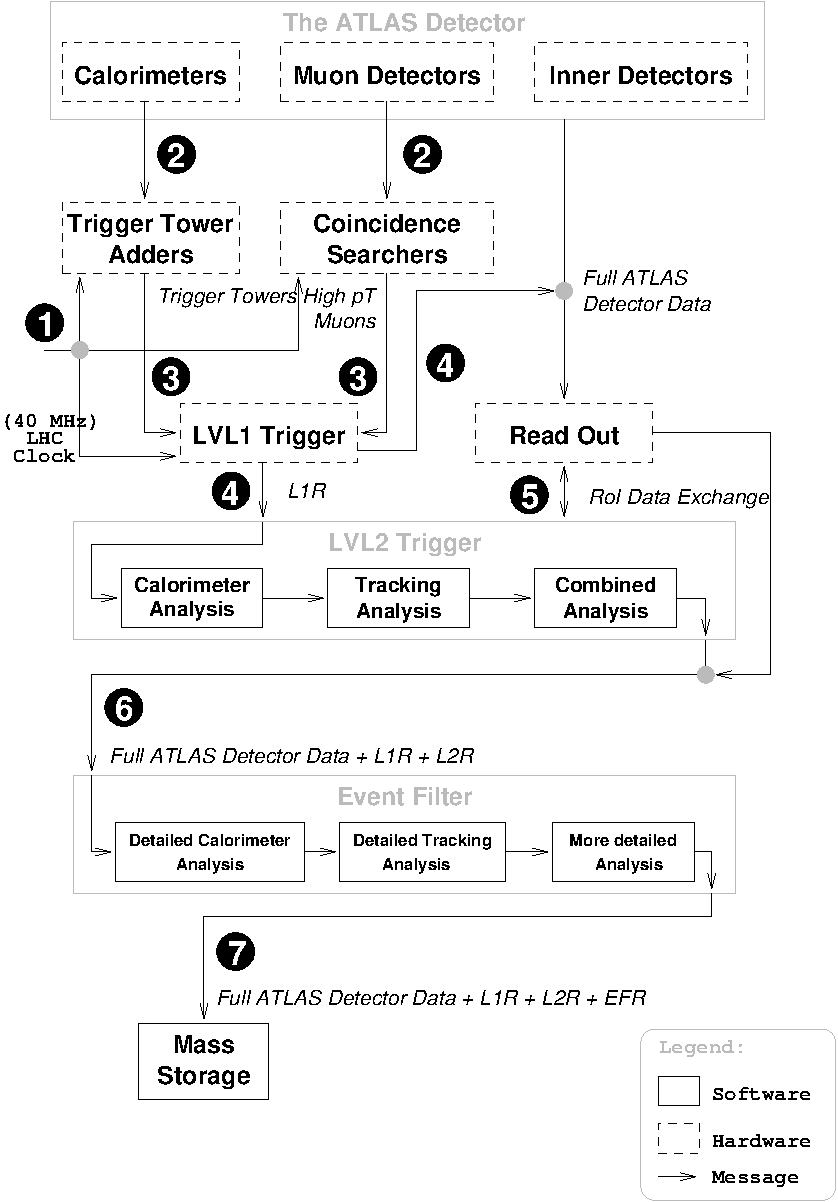
\includegraphics[scale=0.9]{trigger-physics}
\end{center}
\caption{Diagrama esquemático do Sistema de Filtragem do Experimento ATLAS
segundo suas funções de filtragem.}
\label{fig:trigger-physics}
\end{figure}

O processamento começa à medida que o LVL1 recebe o sinal do LHC acusando o
iminente cruzamento de pacotes (do inglês \eng{Bunch Crossing}) no ponto de
impacto. Uma janela de aquisição de alguns nanossegundos fará com que o
Sistema de Leitura do Detetor registre o evento. Os sistemas de
pré-processamento do LVL1 são ativados paralelamente. No caso dos
Calorímetros, somadores rápidos \cite{seixas:adder} agrupam as informações das
células dos calorímetros e.m. e hadrônicos, formando 2 planos com
granularidade reduzida \cite{l1-tdr}. Em ambas seções do calorímetro (e.m. e
hadrônica) este pré-processamento forma macro-células de filtragem ou
``torres" de filtragem (do inglês, \eng{Trigger Towers}, ou TT) com tamanho
$0,1\times0,1$ no plano $\eta\times\phi$. As diversas sub-camadas de cada
seção do calorímetro são colapsadas em um único plano por seção. Estes planos
com granularidade minimizada são varridos pelos diversos processadores do LVL1
e os objetos de interesse localizados no detetor. Para a deteção de um objeto
tipo e.m. requer-se normalmente que perceba-se pouca (ou nenhuma) energia na
seção hadrônica e que grande parte da energia do objeto esteja concentrada
numa região $0,2\times0,2$ ao redor do ponto estimado de impacto
(isolamento). A energia deste núcleo deve ser maior que o corte imposto pelo
sistema de filtragem; no atual caso de estudo, 25 GeV ao menos. Os valores de
corte e isolamento são configuráveis.

É interessante perceber que múltiplas assinaturas podem ser detetadas em um
único evento para além do fato de que múltiplas RoI's secundárias possam estar
presentes. Uma lista das assinaturas encontradas e das diversas RoI's
averiguadas pelo LVL1 são repassadas para o LVL2, no formato de uma única
mensagem conhecida como o ``Resultado do Primeiro Nível de Filtragem", ou L1R,
como visto na Seção~\ref{sec:lvl2arch}. No caso da assinatura sendo estudada,
ao menos uma RoI primária, indicando um objeto tipo e.m., com ao menos 25 GeV
estará presente no L1R.

O processamento no LVL2 é seqüencial. Ao receber um L1R, o Guia de Execução do
LVL2 (do inglês, \eng{Steering}) chamará um componente para a confirmação do
disparo do LVL1. O componente em questão poderá transferir do Sistema de
Leitura do Detetor, a quantidade de dados que achar necessária, ao redor da
RoI, para processá-la. Se não for possível rejeitar a assinatura do LVL1, o
\eng{Steering} poderá chamar mais e mais componentes até que o evento seja
rejeitado ou definitivamente aprovado ao Terceiro Nível de Filtragem ou Filtro
de Eventos (do inglês \eng{Event Filter} ou EF). Neste último caso, de forma
equivalente a relação entre o LVL1 e o LVL2, o LVL2 enviará um sumário
indicando a razão da aceitação do evento, e valores refinados de energia,
momento e localização dos objetos explorados em seu contexto ao EF. Espera-se
que o LVL2 atinja uma redução da taxa de eventos, dos 25~kHz inicialmente
cedidos pelo LVL1 para não mais que alguns (1 ou 2) kHz. O tempo médio de
processamento deve estar na ordem dos 10~ms. Note que este valor representa a
média de processamento por evento. De fato espera-se que eventos de interesse
utilizem mais tempo de processamento enquanto que eventos pouco ou nada
interessantes sejam rapidamente descartados.

Neste contexto entende-se que, quanto menor o tempo necessário e maior a
qualidade da deteção dos diversos componentes do sistema de filtragem, mais
tempo computacional será despendido com a Física de interesse e menos recursos
com eventos que representem Física ordinária ou incorretamente detetada.

No EF a análise do evento começa com 100\% dos dados do evento e os resultados
dos nível precedentes (L1R e L2R). Neste nível de filtragem, correlações mais
complexas podem ser feitas entre as diferentes RoI's, e uma análise mais
depurada do evento poderá ser conduzida. Por exemplo, é possível se fazer uso
das RoI's secundárias para atingir maior redução da taxa de eventos a ser
registrada em mídia permanente. Se aprovado, o evento é guardado, devidamente
``etiquetado" e repassado às fazendas de processamento \eng{offline} para
posterior reconstrução.

\paragraph{Contaminação} O \eng{trigger} de elétrons ou fótons conterá forte
contaminação de jatos com poucas componentes hadrônicas, difícil de deteção
observando-se a granularidade disponível no LVL1. Somente no LVL2, o Sistema
de Filtragem, disporá do tempo e da completa granularidade do detetor para
executar uma seleção mais criteriosa. Estima-se em \cite{daqnote00-02}, que a
cada 25.000 objetos do tipo e.m., aprovados pelo LVL1, apenas 1 será um
elétron ou fóton.

\section{Deteção de elétrons baseada em Calorimetria}
\label{sec:e-detection}

A Figura~\ref{fig:e-shower} mostra a interação de um elétron com um detetor de
traços (\eng{Cloud Chambers}) e absorvedores de chumbo. Nesta figura é
possível observar a formação de um chuveiro de partículas que diverge
aproximadamente isotropicamente do eixo de penetração do elétron. No caso de
elétrons \cite{wigmans-book}, a dispersão é menor que no caso de jatos de
partículas, já que há uma grande probabilidade de espalhamento múltiplo (do
inglês \eng{Multiple Scattering}) causado pelas componentes hadrônicas do
conjunto de partículas. A distância de penetração é diretamente proporcional a
energia do objeto em análise \cite{leo, knoll}, ainda que, para os mesmos
valores energéticos, jatos tendam a penetrar mais profundamente nos aparatos.

\begin{figure}
\begin{center}
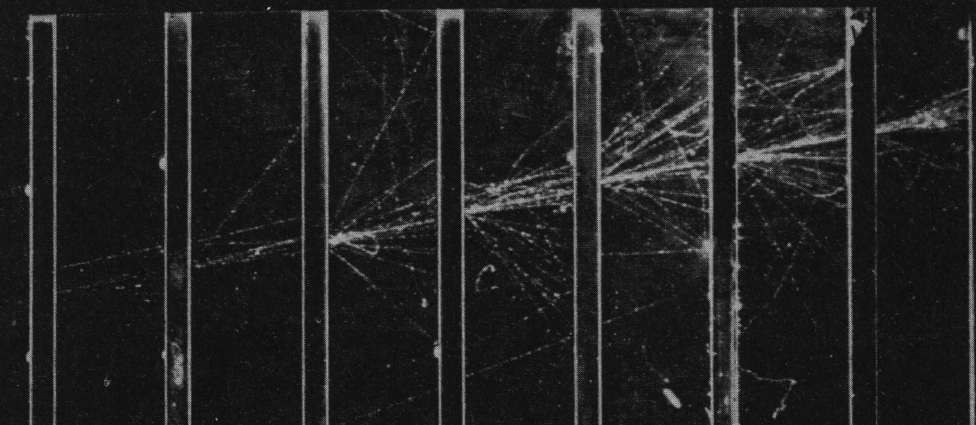
\includegraphics[scale=0.4]{e-cloud-chamber}
\end{center}
\caption{Interação de um elétron com um detetor de traços com absorvedores em
chumbo.} 
\label{fig:e-shower}
\end{figure}

%%CONSEGUIR FOTO DE UMA ROI COM O DÊNIS: ELECTRON, JET?

A deteção de elétrons beneficia-se deste conhecimento básico para
distingui-los de sua contaminação natural de jatos (e píons). Numa primeira
fase, chamada de Extração de Características, avalia-se para uma região do
detetor, normalmente centralizada em um ponto pré-determinado, um conjunto de
valores que representem, o melhor possível, os perfis de deposição lateral (ou
radial) do objeto sendo estudado e sua penetração no aparato. Este processo
comprime\footnote{Define-se ``compressão" a técnica pelo qual reduz-se a
dimensionalidade de um sinal em um espaço bem definido, preservando ou
tentando preservar a informação relevante que caracteriza este sinal de
interesse. A transformação do espaço original para o espaço ``comprimido" é
irreversível. A ``compressão" de sinais é muitas vezes denominada
``compactação com perdas".} a informação de entrada, que normalmente possui
dimensionalidade bastante elevada (O(100)-O(1000)), para um conjunto pequeno
(O(10)) de variáveis que possam ser analisadas mais facilmente.

A questão da dimensionalidade da entrada está intimamente correlacionada com a
capacidade discriminatória do calorímetro. Quanto mais granular, maior precisão
pode ser obtida na definição de pontos de impacto e deteção de partículas. O
revés é o custo - detetores multi-segmentados são mais difíceis e caros de
serem construídos.

No caso do experimento ATLAS (veja a Seção~\ref{sec:atlas-calo} para mais
detalhes), os calorímetros são segmentados em diversas camadas, e, camada a
camada, granularizados em células de deposição energética. A granularidade
varia camada a camada pois cada uma delas possui um objetivo distinto de
emprego: as camadas iniciais tem por objetivo a discriminação de elétrons e
fótons e estimativa de posicionamento, as mais traseiras a deteção de
hádrons. As camadas da seção e.m. tem profundidade variante, sendo que a
segunda (EM2, a contar do zero, ou seja o pré-irradiador), tem a maior
profundidade de todas, ocupando mais de 80\% do volume total desta seção.

Para elétrons com valores energéticos até algumas dezenas de
gigaelétron-volts, espera-se que a maior parte da energia do objeto esteja
depositada nesta camada. A granularidade é bastante regular e semelhante tanto
ao longo do eixo $\eta$ quanto ao longo de $\phi$, como é possível observar na
Tabela~\ref{tab:lar}. Esta tabela também mostra o fator de compressão (ou
tamanho da torre de filtragem) $N_{\eta} \times N_{\phi}$ aplicado ao processo
de agrupamento necessário ao pré-processamento antes da análise encaminhada
pelo LVL1.

A seção hadrônica dos calorímetro é bastante menos granular. O tamanho padrão
da célula é $0,1\times0,1$ no espaço $\eta\times\phi$ uma vez que seja
otimizado para detetar hádrons. Esta classe de partículas penetra mais
profundamente na matéria e desenvolve complexas cascatas ao longo da
penetração, normalmente pouco interessantes, mais que devam ser contidas no
espaço do detetor. O agrupamento padrão (torre de filtragem) para LVL1 é de
$2\times2$ células.

A Figura~\ref{fig:e-jet-deposit} mostra histogramas da relação da deposição
energética na seção hadrônica e a energia total do objeto considerando-se uma
área $0,4\times0,4$ no plano $\eta\times\phi$. Os eventos considerados são
simulações de elétrons e jatos cobrindo um campo energético de algumas dezenas
de GeV até 90 GeV interagindo com os calorímetros do ATLAS. Os eventos
selecionados passaram uma simulação realística do LVL1 e portanto representam,
todos, eventos que seriam classificados como elétrons por este nível de
filtragem. Observa-se que para jatos há uma probabilidade maior de depósito na
seção hadrônica que na seção e.m..

\begin{figure}
\begin{center}
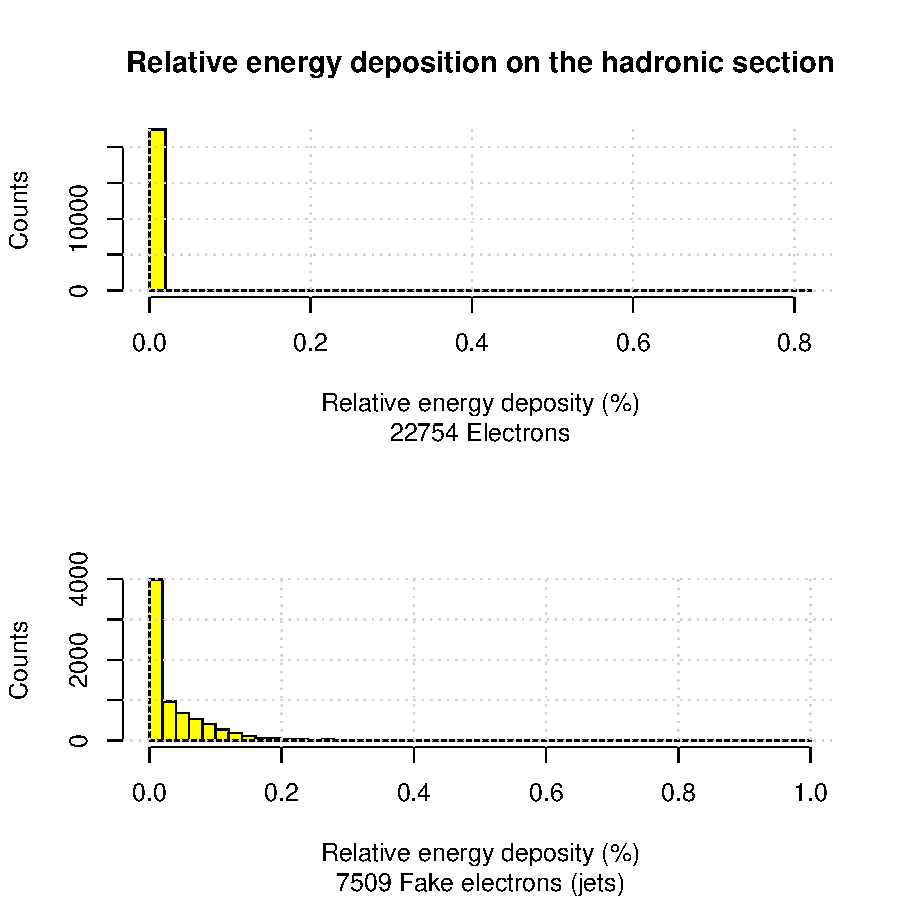
\includegraphics[scale=0.95]{em-had-percent}
\end{center}
\caption{A relação energética da deposição na seção hadrônica e energia total para
elétrons (topo) e jatos (baixo).}
\label{fig:e-jet-deposit}
\end{figure}

\paragraph{Classificação -} A fase seguinte à compressão do espaço original
de entrada é a discriminação da Física de interesse. Tipicamente
\cite{hlt-tdr, zeus-neural} a deteção é realizada por meio da definição de
patamares de separação (também ditos \emph{cortes}) com informação \emph{a
priori} \cite{vantrees}. Este trabalho é normalmente realizado por um físico
experiente, de acordo com a importância da física de interesse analisada. 

É importante salientar que o melhor classificador baseado em cortes cortes com
informação \emph{a priori} também pode ser atingido iterativamente através de
utilização de Discriminadores de Fisher \cite{haykin-adaptative},
opcionalmente com atribuição de pesos para cada classe de partículas,
definindo importâncias diferentes aos diferentes tipos de objetos estudados.

A Figura~\ref{fig:basic-discriminator} mostra um diagrama esquemático do
processo clássico de deteção descrito. No centro lógico do processo
encontra-se o físico experiente, que controla o grau de compressão e
capacidade discriminatória do sistema. Este sistema possui um conjunto de
problemas inerentes a intervenção humana na otimização, dentre eles a
dependência no operador (aqui representado pela figura do "físico
experiente"). O procedimento de compressão e discriminação deve ser bem
documentado para que seja possível a reprodução dos resultados em todos os
momentos. Ademais, o ajuste fino poderá ser bastante tedioso e dependente da
quantidade de dados analisados, uma vez que o processo realizado será
semi-automático - i.e., seleção dos dados de interesse seguido de análise
manual.

\begin{figure}
\begin{center}
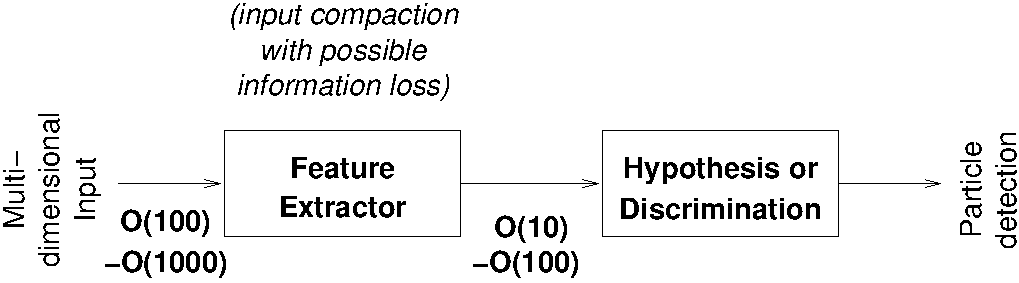
\includegraphics[scale=0.5]{basic-discriminator}
\end{center}
\caption{Um sistema \eng{ad-hoc} de deteção com uma entrada com alta
dimensionalidade.}
\label{fig:basic-discriminator}
\end{figure}

\subsection{Compressão minimizada}

Em um sistema com a dimensionalidade de entrada tão elevada como se apresenta
o problema da discriminação elétron/jato para o Detetor ATLAS, é mais
interessante a proposição de um sistema onde a otimização seja conduzida por
bases matemáticas mais automáticas e maximamente livres de
polarização. Idealmente este sistema utilizaria todas as entradas para definir
as regras de compressão e relevância de cada componente na discriminação dos
alvos. Infelizmente, com o aumento da dimensionalidade da entrada diminui-se
exponencialmente as chances de convergência na procura de uma função que
defina otimamente ou de forma aproximada, uma separação das classes a serem
discriminadas \cite{haykin}. É razoável supor que, quanto maior a
dimensionalidade da entrada, mais dados serão necessários para atingir-se uma
discriminação suficientemente boa. 

Desta forma um sistema de compressão mínima dos dados se faz necessária. Este
sistema de compressão deve tentar minimizar a perda de informação e maximizar
o potencial discriminatório do sistema. Um discriminador capaz de definir um
plano de separação em um espaço de entrada com dimensionalidade elevada também
será necessário, uma vez que deseja-se compressão mínima dos dados de
entrada. A Figura~\ref{fig:advanced-discriminator} mostra uma idealização de
tal sistema de discriminação. A primeira etapa é uma compressão mínima da
entrada, que seja compatível com um sistema de deteção que aceite sinais com
alta-dimensionalidade na entrada. Idealmente, um sub-sistema de ``otimização"
dos parâmetros de compressão e discriminação, também automatizado, controlaria
a compressão da entrada melhorando a relação custo computacional \eng{versus}
qualidade de deteção.

\begin{figure}
\begin{center}
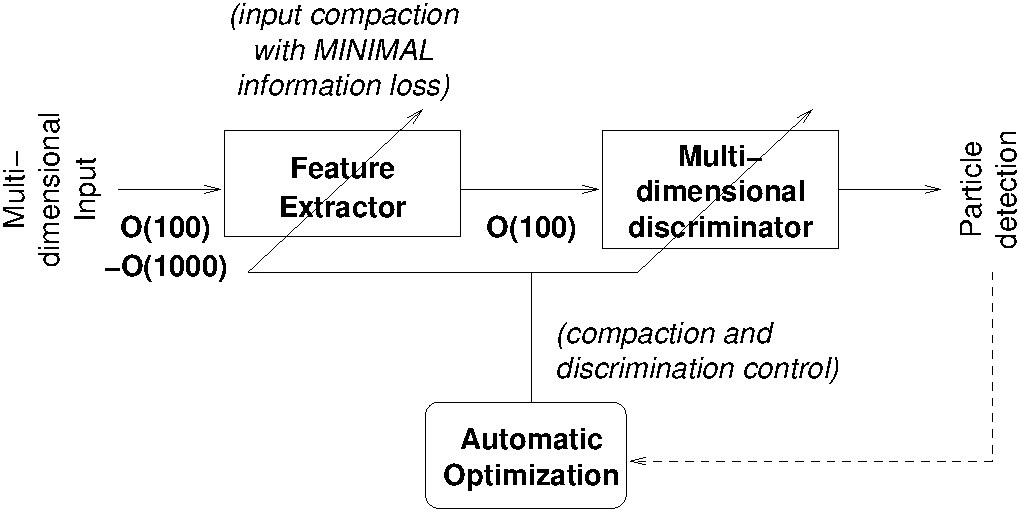
\includegraphics[scale=0.5]{advanced-discriminator}
\end{center}
\caption{Um sistema \eng{ad-hoc} de deteção sub-ótimo com uma entrada com alta
dimensionalidade.}
\label{fig:advanced-discriminator}
\end{figure}

\section{Deteção de Elétrons no LVL2}
\label{sec:lvl2-detect-electron}

O LVL1 (Seção~\ref{sec:lvl1}) executa seu procedimento de filtragem procurando
elementos nos calorímetros e detetores de múons que obedeçam a certos
critérios de classificação. A Tabela~\ref{tab:l1-rates} mostrada anteriormente
indica os principais objetos interessantes neste nível de filtragem. No caso
de objetos e.m. (elétrons e fótons), o algoritmo pode ser resumido da seguinte
forma:

\begin{enumerate}
\item Os sinais analógicos provenientes das células do detetor são agrupados
em macro-células chamadas Torres de Filtragem (do inglês \eng{Trigger Towers},
TT). A taxa de agrupamento não é uniforme, mas num geral forma TT's com
$0,1\times0,1$ no plano $\eta\times\phi$ para a seção eletromagnética do
calorímetro e $0,2\times0,2$ na seção hadrônica.

\item Os sinais somados das TT's são digitalizados e disponibilizados para a
lógica de leitura do LVL1;

\item Processadores especializados (4 no total) cobrem diferentes áreas do
detetor e utilizam um algoritmo de agrupamento baseado em uma janela
deslizante \cite{l1-tdr} cobrindo uma região de $4\times4$ TT's (16 no
total) aqui resumido:

\begin{enumerate}
\item Se o núcleo de $2\times2$ TT's contiver energia maior que a
periferia, para um determinado patamar programável, um candidato a RoI é
definido;

\item Em seguida soma-se, duas a duas, as energias transversas das TT's do
núcleo de $2\times2$ TT's e utiliza-se a maior das somas em uma comparação com
um patamar de energia EM;

\item Caso passe a este critério, a energia na periferia da RoI-candidata é
verificada para assegurar o isolamento do objeto; 

\item O último critério é o isolamento hadrônico onde o LVL1 verifica se não
há grande depósito de energia (transversa) na seção hadrônica.
\end{enumerate}  

No caso de atender a todos os pré-requisitos, o objeto candidato é promovido a
uma RoI tipo e.m.. Este algoritmo está representado na
Figura~\ref{fig:l1-calo}.
\end{enumerate}

\begin{figure}
\begin{center}
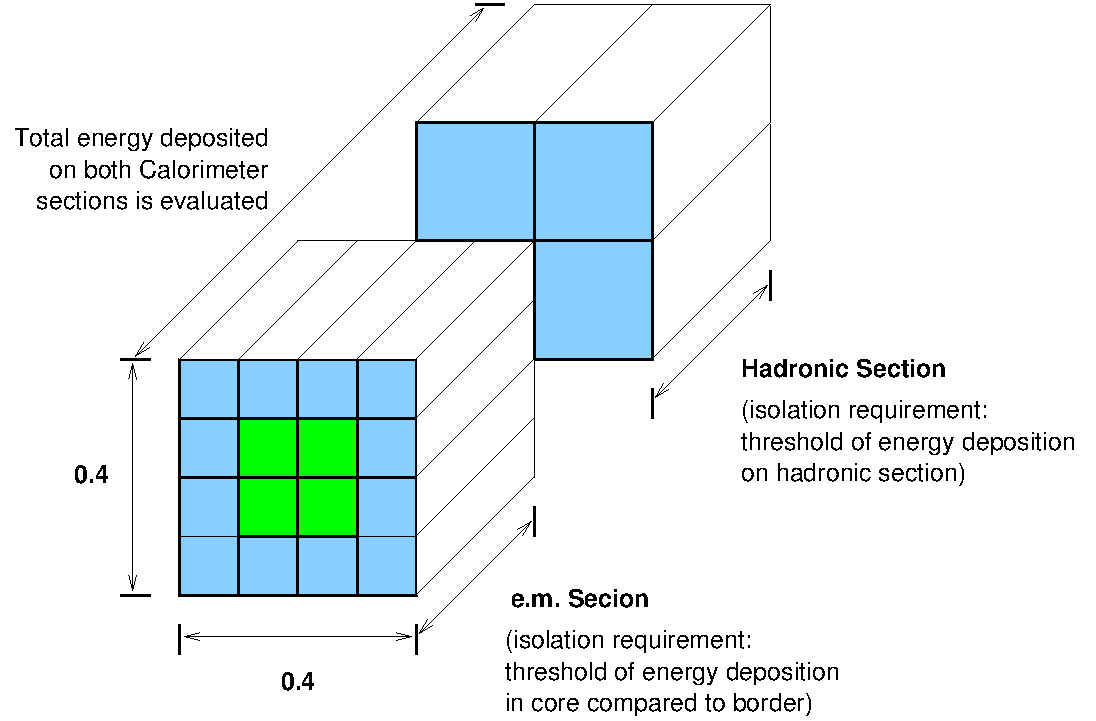
\includegraphics[scale=0.78]{l1-calo}
\end{center}
\caption{Representação gráfica do algoritmo de deteção de objetos e.m. no LVL1.}
\label{fig:l1-calo}
\end{figure}

Os diversos sub-módulos do LVL1 irão detetar e pré-classificar os elementos de
interesse para jatos, múons e energia faltante. Em seguida:

\begin{enumerate}
\item Os objetos detetados e seus pontos \textbf{centrais} de impacto
estimados no plano $\eta\times\phi$, ou seja, as RoIs, são encaminhados ao
Processador Central do Sistema de Filtragem do LVL1 (do inglês \eng{Central
Trigger Processor}, CTP) e uma decisão é feita levando-se em consideração as
assinaturas de interesse e resultados dos processamentos de outros módulos
(jatos, energia faltante e múons). A decisão de aprovar um evento é tomada
baseando-se em RoI's de acordo com critérios de preferência estipulados \eng{a
priori}. As RoI's que são utilizadas para a decisão de aprovação são rotuladas
``primárias" ao passo que as demais, ``secundárias";

\item Um sumário do resultado e das RoI's encontradas, já rotuladas (primárias
e secundárias) é repassado, através do \eng{RoI Builder} ao LVL2.
\end{enumerate}

O Segundo Nível de Filtragem do experimento ATLAS é a primeira vez onde o
evento será analisado tendo por base a granularidade máxima do detetor. O
objetivo deste nível de filtragem, de uma forma geral, é a confirmação das
informações do LVL1 e eventual depuração e extensão. Aproveitando-se de toda
a granularidade disponibilizada pelo sistema de leitura do detetor, o LVL2
começa analisando o evento através das RoI's classificadas como primárias pelo
LVL1.

Ao receber as informações das RoI's o \eng{Steering} ativará o passo de
decodificação do resultado do LVL1 e, em seguida, selecionará a próxima fase
de análise, que dependerá diretamente do tipo RoI's primárias do evento. No
caso de RoI's do tipo e.m., um algoritmo de deteção de elétrons (e fótons)
será ativado.

\subsection{Deteção de elétrons no LVL2: O T2Calo e EGammaHypho}
\label{sec:classic-detection}

Como discutido anteriormente na Seção~\ref{sec:e-detection}, o processo de
deteção veloz baseado em calorimetria pode ser sub-dividido em passos distintos:

\begin{enumerate}
\item Compressão do sinal de entrada;
\item Deteção da física de interesse baseada no espaço comprimido.
\end{enumerate}

Para o ATLAS, a fase 1 irá comprimir o espaço de entrada definido pelas
células da RoI em questão em 4 variáveis com alto poder discriminatório, baseado
na percepção da física de interesse e da contaminação esperada. No caso de
elétrons, espera-se que haja forte contaminação de jatos com muitas
componentes e.m.. Desta forma, a compressão do sinal de entrada tentará
realçar informações como a dispersão do objeto na RoI ou a profundidade de
interação do objeto com as diversas camadas do detetor. 

O nome do algoritmo usado para a FEx de RoI's primárias tipo e.m. é
\emph{T2Calo}, uma variação das palavras \eng{Trigger}, LVL2 e
Calorimetria. As variáveis extraídas do \eng{cluster} definido pela RoI do
LVL1, por este algoritmo, são, em ordem:

\begin{enumerate}
\item \textbf{Centro de Impacto Refinado}, Figura~\ref{fig:t2calo-1}: O
primeiro passo do algoritmo é um refinamento do centro da RoI. Isto é feito
encontrando-se o pico de deposi\-ção ener\-gé\-tica na segunda camada da
se\-ção eletroma\-gné\-tica do calo\-rí\-metro, que é tam\-bém a mais profunda
(veja uma discus\-são mais detalhada em~\ref{sec:atlas-calo}) desta se\-ção. O
valor do centro da cé\-lula é tomado como nova estimativa de posicionamento da
RoI e será utilizado para os cál\-culos seguintes;

\item \textbf{$\text{Energia}^{e.m.2}_{3 \times 7}$},
Figura~\ref{fig:t2calo-1}: O segundo passo é calcular as somas dos valores de
deposição energética, para a segunda camada e.m., numa região de tamanho
$\eta=0,075 \times \phi=0,175$ ao redor do centro de impacto definido
anteriormente. Esta soma é assim designada devido à granularidade de base da
segunda camada e.m., para cada célula, de aproximadamente $0,025 \times
0,025$;

\item \textbf{$\text{Energia}^{e.m.2}_{3 \times 7}$},
Figura~\ref{fig:t2calo-1}: Em seguida calcula-se as somas dos valores de
deposi\-ção ener\-gé\-tica, para a segunda camada e.m., numa região de tamanho
$\eta=0,175 \times \phi=0,175$ ao redor do centro de impacto definido no
primeiro passo;

\begin{figure}
\begin{center}
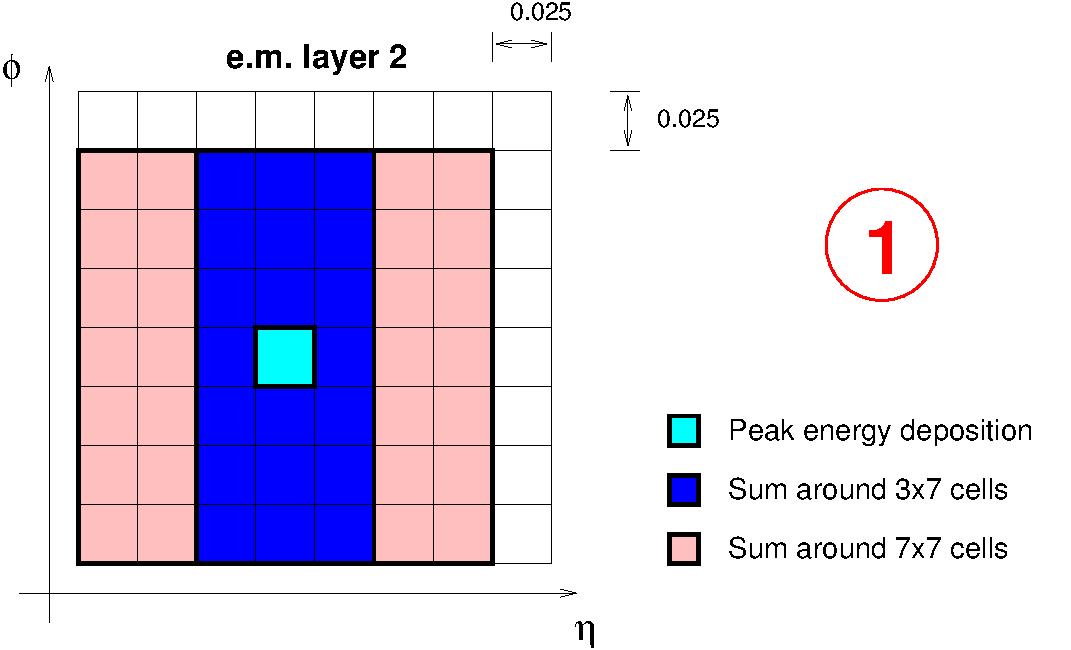
\includegraphics[scale=0.8]{t2calo-1}
\end{center}
\caption{T2Calo, Etapa 1: Cálculo do centro refinado e deposições de
energia na segunda camada e.m., para regiões $3\times7$ e $7\times7$ no plano 
$\eta\times\phi$.}
\label{fig:t2calo-1}
\end{figure}

\item \textbf{Máximos em e.m.1}, Figura~\ref{fig:t2calo-2}: Os dois maiores
picos de energia na primeira camada da seção e.m. são detetados;

\begin{figure}
\begin{center}
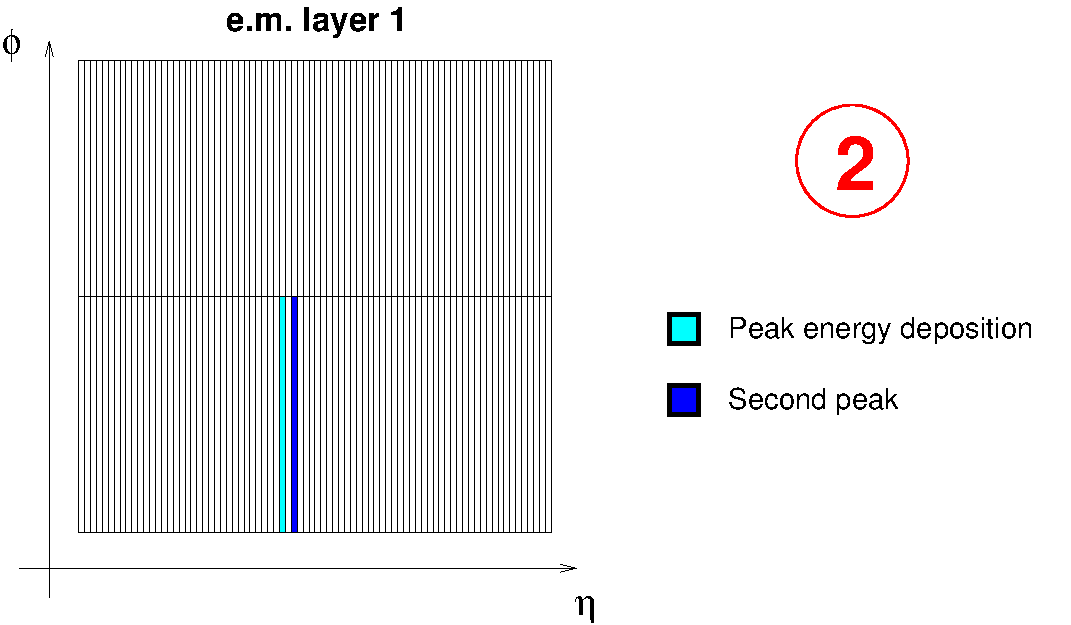
\includegraphics[scale=0.8]{t2calo-2}
\end{center}
\caption{T2Calo, Etapa 2: Procura dos dois maiores picos na primeira camada e.m..}
\label{fig:t2calo-2}
\end{figure}

\item \textbf{Energia e.m.}, Figura~\ref{fig:t2calo-3}: Embora não utilizados
diretamente para o processo discriminatório, os valores parciais de deposição
energética para cada camada da seção e.m., numa região de $\eta=0,075 \times
\phi=0,175$, também são calculados;

\begin{figure}
\begin{center}
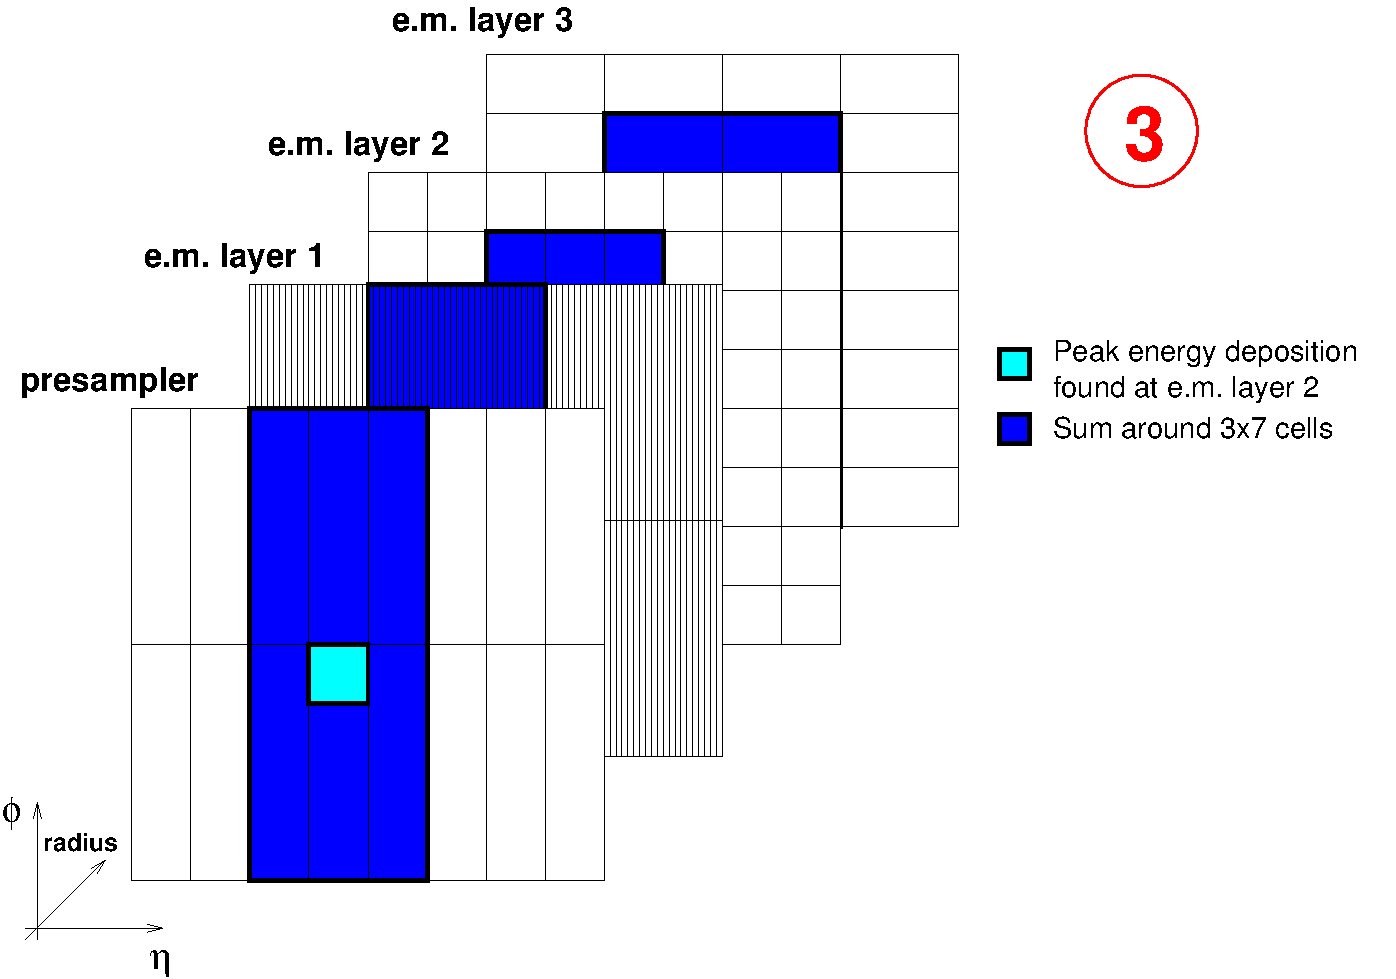
\includegraphics[scale=0.6]{t2calo-3}
\end{center}
\caption{T2Calo, Etapa 3: Valores parciais e somatório das energias, em uma
área equivalente a $3\times7$ células na segunda camada e.m., para as demais
camadas da seção e.m..}
\label{fig:t2calo-3}
\end{figure}

\item \textbf{$\text{Energia Hadrônica}_{2 \times 2}$}: Calcula-se a energia
total num espaço $\eta=0,2 \times \phi=0,2$ tomando-se os valores das células
cujo o centro recai sobre a região definida em cada camada da seção hadrônica;

\begin{figure}
\begin{center}
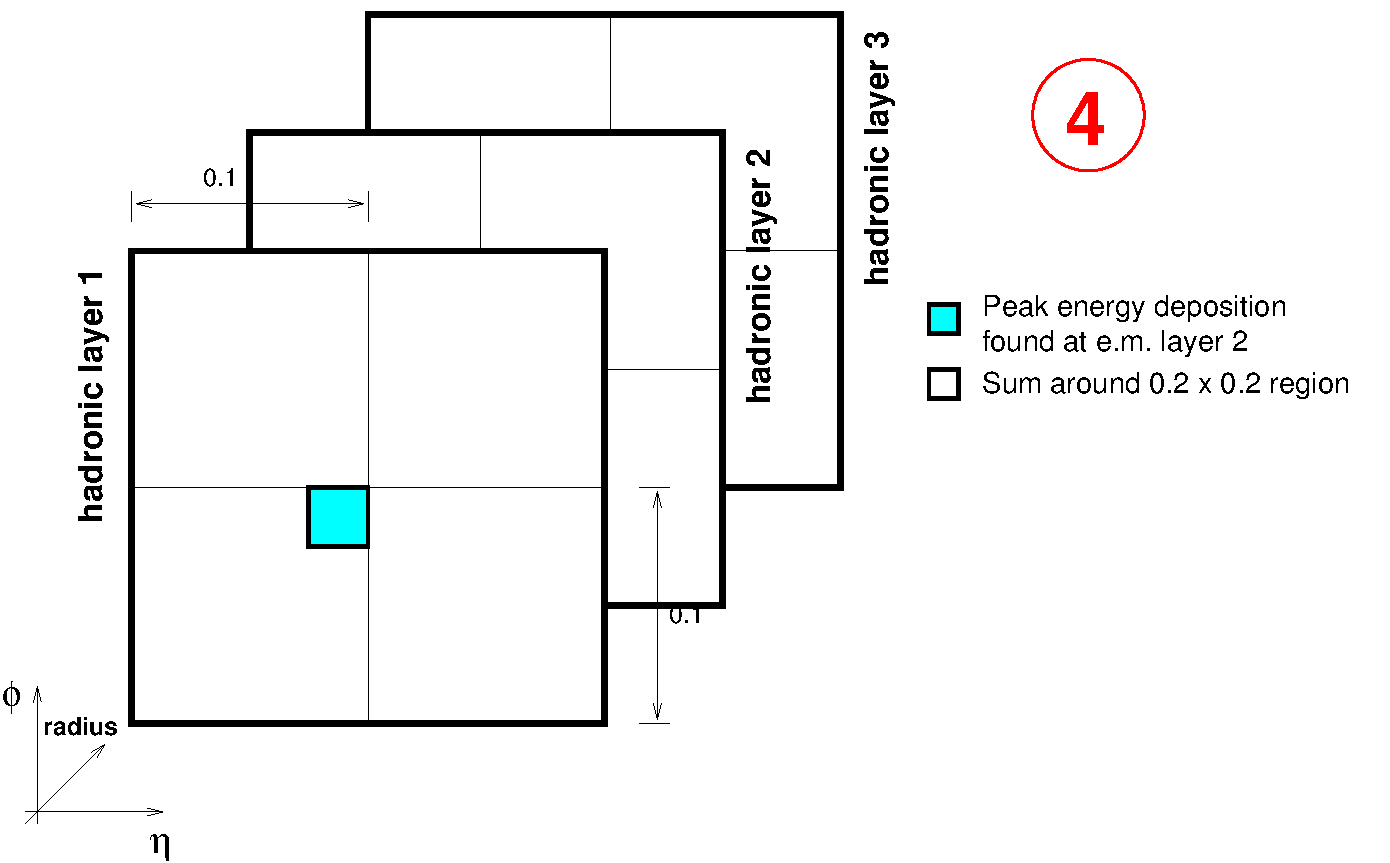
\includegraphics[scale=0.6]{t2calo-4}
\end{center}
\caption{T2Calo, Etapa 4: Valores parciais e somatório das energias, em uma
área equivalente a $0,2\times0,2$ no plano $\eta\times\phi$, para as camadas
da seção hadrônica.} 
\label{fig:t2calo-4}
\end{figure}

\end{enumerate}

O algoritmo de deteção propriamente dito segue a execução do T2Calo e é
chamado \emph{EGammaHypho}. Este algoritmo tem a função exclusiva de combinar
as informações disponíveis dos diversos algoritmos de FEx relacionados à
deteção de elétrons e fótons e tomar uma decisão simples baseada nas
propriedades físicas das partículas de interesse. No caso de RoI's tipo e.m.,
o EGammaHypho é também executado logo após a execução do T2Calo visando uma
rejeição rápida da física responsável pelo ``ruído" (ou \eng{background}), ou
seja, jatos. As vantagens deste processo de rejeição ``antecipada" foram
discutidas no Capítulo~\ref{chap:trigger}.

Uma vez que a quantidade de informações disponível neste momento encontra-se
somente nos parâmetros pré-definidos pelo T2Calo, o EGammaHypho definirá uma
seqüência simples de discriminadores baseados em combinações lineares e
não-lineares destas quantidades. As quantidades de interesse do EGammaHypho
são: 

\begin{enumerate}
\item \textbf{Centros refinados da RoI}: Procurando-se o pico de deposição
energética na segunda camada e.m., utilizando a granularidade máxima do
detetor, é possível refinar o ponto de impacto do objeto. Estes valores serão
utilizados para o cálculo das demais variáveis do T2Calo;

\item \textbf{\rcore}: Representa a razão entre a soma das células na segunda
camada e.m., numa área de $3 \times 7$ células por $7 \times 7$ células ao
redor da célula na segunda camada que apresenta o maior valor de energia
depositado, como calculado na Etapa~1 do T2Calo. Esta quantidade mede o
espalhamento da cascata formada pelo decaimento do objeto de estudo. No caso
do objeto ser um jato, espera-se que a cascata tenha um espalhamento maior que
no caso de elétrons, resultando em um valor menor que 1 para esta quantidade;

\item Cálculo de \textbf{\eratio}: Uma vez que jatos de par\-tí\-culas
interagem de forma mais espalhada do que e\-lé\-trons, espera-se que na
primeira camada e.m. sejam observados vários picos. Definindo um pico ($E$)
como sendo a ocorrência de um máximo registrado pela célula central de um
agrupamento de três células adjacentes, então, a quantidade \eratio\
representa a razão de energias \eratio$=\frac{E_1-E_2}{E_1+E_2}$. Ou seja, a
razão da subtração pela soma dos valores de energia dos dois picos mais
energéticos na primeira camada e.m., como calculado na Etapa~2 do T2Calo.

Se o objeto for um elétron (objeto único), espera-se que $E_2=0$, já que a
cascata de partículas que o elétron forma na sua interação com o calorímetro
é, tipicamente, bastante estreita, e portanto \eratio=1. Para jatos,
normalmente, \eratio\ será menor que 1, já que $E_2 \neq 0$;

\item \textbf{\etem}: Esta quantidade representa a soma das energias das
células da seção e.m. dos calorímetros, cujo centro recai sobre uma região de
$0,075 \times 0,175$ no plano \ep, ao redor do centro da célula da segunda
camada e.m. que apresenta o maior valor de energia depositada, como calculado
na Etapa~3 do T2Calo. O valor original calculado é dividido pelo
$\cosh{|\eta|}$ para que obtenha-se a energia transversa\footnote{O termo
``transverso" neste contexto refere-se ao feixe de partículas.} (projetada no
plano $x \times y$ do detetor). A região na qual esta quantidade é extraída
equivale, usando-se a granularidade da segunda camada e.m., a uma região de 3
células na direção $\eta$ por 7 células na direção de $\phi$. Espera-se que a
energia de elétrons esteja totalmente contida nesta janela; por seu turno,
jatos devem apresentar, hipoteticamente, uma fração menor de sua energia
depositada nesta área;

\item \textbf{\ethad}: Esta quantidade representa a soma das células na
primeira camada da seção hadrônica do calorímetro dentro de uma região de $0,2
\times 0,2$ no plano \ep, ao redor do centro da célula na segunda camada
e.m. que apresenta o maior valor de energia depositada, como calculado na
Etapa~4 do T2Calo. O valor também é divido por $\cosh{|\eta|}$ para que
obtenha-se o valor de energia transversa. Para elétrons, a quantidade de
energia depositada na camada hadrônica deve ser próxima de zero, enquanto que,
para jatos, espera-se que seja diferente de zero.
\end{enumerate}

A seqüência discriminatória está representada a seguir, em pseudo-código:

\newcommand{\textbu}[1]{\textbf{\underline{#1}}}
\newcommand{\IF}[1]{\textbu{se} #1, \textbu{então}}
\newcommand{\RETURN}[1]{\\ \textbu{retornar} #1\textbf{;}}
\newcommand{\EVALTWO}[3]{\textbu{calcular} #1(#2, #3)\textbf{;}}
\newcommand{\lumihi}{\ensuremath{10^{33} \text{cm}^{-2}\text{s}^{-1}}}

\begin{description}
\item[\ding{182}] \EVALTWO{\eratio}{$E_1$}{$E_2$}
\item[\ding{183}] \EVALTWO{\rcore}{$\text{Energia}^{e.m.2}_{3\times7}$}{$\text{Energia}^{e.m.2}_{7\times7}$}
\item[\ding{184}] \EVALTWO{\etem}{Energia e.m.$_{3\times7}$}{$|\eta|$}
\item[\ding{185}] \EVALTWO{\ethad}{Energia had.$_{0,2\times0,2}$}{$|\eta|$}

\item[\ding{186}] \IF{centro da RoI em e.m.2 distante ($\gtrapprox 0,1$) do
definido pelo LVL1}
	\RETURN{\textbf{não é} elétron}

\item[\ding{187}] \IF{$\rcore \lessapprox 0,9$}
	\RETURN{\textbf{não é} elétron}

\item[\ding{188}] \IF{$\eratio \lessapprox 0,75$}
	\RETURN{\textbf{não é} elétron}

\item[\ding{189}] \IF{$\etem \lessapprox 25$ GeV, L = \lumihi}
	\RETURN{\textbf{não é} elétron}

\item[\ding{190}] \IF{$\ethad \gtrapprox 1$ GeV, L = \lumihi}
	\RETURN{\textbf{não é} elétron}

\end{description}

Se o objeto definido pelo LVL1 conseguir passar todos os critérios definidos
neste procedimento, é promovido a ``candidato à elétron" dentro do LVL2. As
fases seguintes de discriminação tentarão encontrar um traço, com momento
equivalente a energia do \eng{cluster}, e uma nova rodada de hipóteses
confirmará (ou não) o elétron. A procura de traços nos detetores internos é um
procedimento tipicamente lento (na ordem de dezenas, dependendo centenas de
milissegundos \cite{hlt-tdr}), e deve ser evitada tanto quanto possível. Por
outro lado, deseja-se que o sistema de deteção preliminar, baseado em
calorimetria seja o mais rápido possível, mas mantendo bons níveis de
discriminação como já discutido.

Uma das estratégias em consideração atualmente, pondera sobre a utilização dos
diversos estágios de hipótese de forma seqüencial, durante a extração de
característica. Neste caso, após interagir com a segunda camada e.m., o T2Calo
seria brevemente parado e a primeira das hipóteses verificada, criando
recursos para uma rejeição ainda mais antecipada. Em seguida, os dados da RoI
para a primeira camada e.m. seriam carregados no processador, a segunda
variável seria calculada e mais uma rodada de decisão seria tomada. As
próximas etapas seriam a carga dos dados da terceira camada e.m. e do
pré-irradiador, seguindo-se da análise de dados na seção hadrônica. 

\subsubsection{Ajuste fino para cada canal}

Para cada uma das assinaturas de interesse aprovadas pelo LVL1, o segundo
nível contará com algoritmos e sistemas de hipótese adequados àquela física. É
interessante notar que mesmo para os canais similares, e.g. (veja a
Tabela~\ref{tab:l1-rates}) \texttt{EM25i} e \texttt{EM15i}, os cortes impostos
pelo algoritmo de hipótese serão otimizados para estas categorias de
energia. 

%Neste trabalho estaremos comparando os diversos algoritmos de deteção
%utilizando um conjunto de eventos destinado ao estudo da discriminação
%elétron/jato no contexto da assinatura mais freqüente do experimento:
%\texttt{EM25i}.

\subsection{Caracterização do T2Calo e do EGammaHypho}
\label{sec:def-eghypo}

Para a caracterização de operação do T2Calo e do algoritmo de hipótese
associado, o EGammaHypho, os seguintes grupamentos de dados foram
considerados:

\begin{itemize}
\item Cerca de 23.000 elétrons simulados via Monte Carlo, proveniente de
interações tipo $H (130 \text{GeV})\rightarrow ZZ \rightarrow 4e^-$ e 
$H (130 \text{GeV})\rightarrow ZZ \rightarrow 2e^- + 2\mu$. Os elétrons de
cada evento simulado interagem com diferentes regiões do detetor;
\item Cerca de 250.000 jatos-duplos, simulados via Monte Carlo, com energia total,
fixa em 25 GeV, também interagindo com várias partes do detetor.
\end{itemize}

Nos dois casos, considerou-se simulações com ruído, proveniente da eletrônica
e uma planta de detetor compatível com o que está sendo instalado atualmente
na caverna do experimento, provendo um ambiente bastante acurado dentro do que
se é possível prever em termos de operação, mas ainda exeqüível em um ambiente
de simulação.

Esta massa original de dados foi submetida a uma simulação do LVL1, que
implementa o algoritmo discutido na Seção~\ref{sec:lvl2-detect-electron},
aceitando todos os eventos com objetos tipo EM com as seguintes
características:

\begin{itemize}
\item ao menos 10 GeV numa região de $2\times2$ torres de filtragem na seção
e.m.;
\item no máximo 4 GeV na região periférica ao núcleo de $2\times2$ torres de
filtragem; 
\item no máximo 2 GeV de depósito na seção hadrônica;
\item qualquer valor para o centro em $\phi$;
\item $\eta$ variando de $-2,5$ a $+2,5$;
\end{itemize}

Um total de cerca de 22.000 elétrons e 7.000 jatos que passariam a um corte
como o proposto acima fazem parte da massa de dados remanescente após as
sanções da simulação do LVL1. A Figura~\ref{fig:transverse-energy} contém os
histogramas de deposição energética total transversa de elétrons (em cima) e
jatos (embaixo), em uma janela de $0,4 \times 0,4$ no plano $\eta\times\phi$,
considerando-se as duas seções do calorímetro (e.m. e hadrônica). É possível
distinguir um corte acentuado nas redondezas de aproximadamente 20~GeV, que
equivale à ação da simulação do LVL1, como esperado. Antes do corte, é
possível distinguir uma cauda, se estendendo até a origem. Este fenômeno pode
ser observado no LVL2 já que os valores de calibração de energia aplicados às
células do calorímetro neste nível de filtragem não estão disponíveis ao nível
de filtragem anterior. Para o histograma de jatos a média aproxima-se ao valor
esperado de 25 GeV, exibindo um pico pronunciado ao redor deste valor. Como é
observa-se, grande parte dos jatos encontram-se com valor de energia
transversa entre 10 e 40~GeV, enquanto que para elétrons, a distribuição decai
suavemente até cerca depois $\approx$ 91~GeV (aproximadamente a massa de
repouso do bóson Z).

% Interessante observar que isto poderá e deverá influenciar nos resultados
% disponíveis, mas o que deseja-se demonstrar é a técnica e não uma solução
% pronta para o problema.

\begin{figure}
\begin{center}
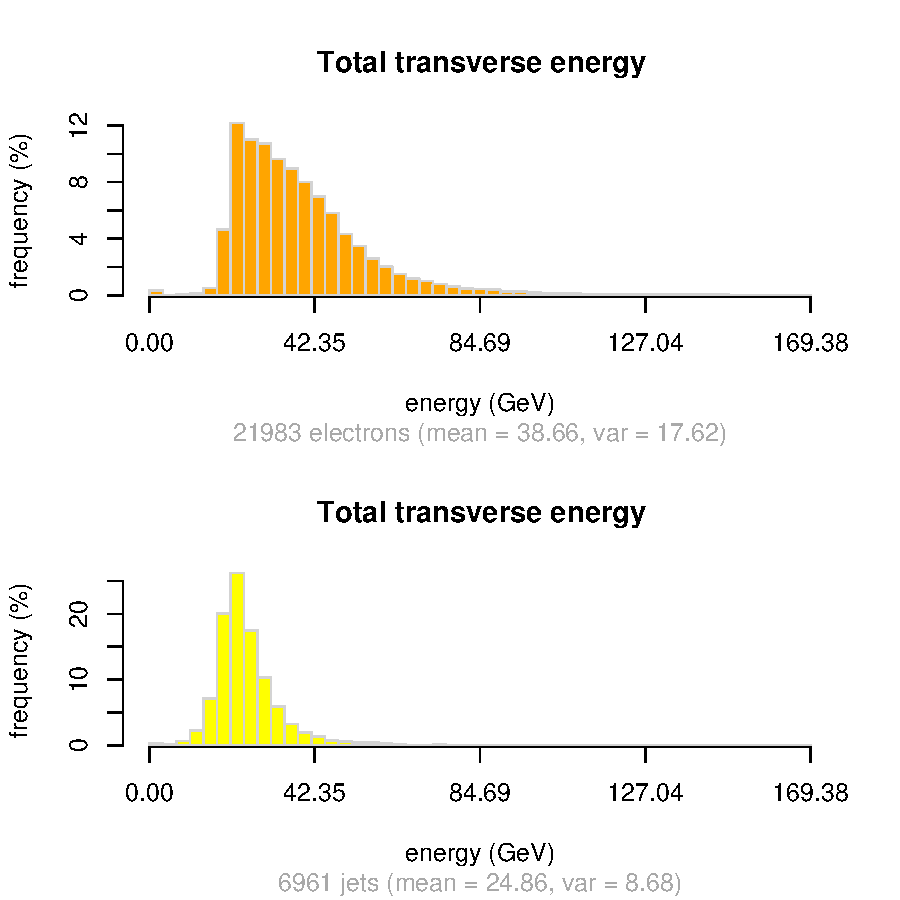
\includegraphics[scale=0.95]{transverse-energy}
\end{center}
\caption{A deposição total de energia em uma região $0,4 \times 0,4$ no plano
$\eta\times\phi$ para elétrons (em cima) e jatos (em baixo) para a massa de
dados disponível para o estudo.}
\label{fig:transverse-energy}
\end{figure}

Nas Figuras~\ref{fig:em-tenergy} e \ref{fig:had-tenergy} observa-se
histogramas da energia transversa total por seção dos calorímetros para
e\-lé\-trons (em cima) e jatos (em baixo). Nota-se que para elétrons, quase
100\% da energia total do objeto é retida na seção e.m., enquanto que para
jatos, nota-se vazamento de energia na seção hadrônica. Embora o corte
realizado pelo LVL1 tenha sido em 2~GeV para o vazamento de energia nesta
seção, observa-se uma quantidade não desprezível de eventos logo após este
valor. Ainda sim, a energia total na seção decai rapidamente e assume-se que a
cauda esteja, mais uma vez, relacionada a qualidade da calibração dos dados
para este nível de filtragem.

\begin{figure}
\begin{center}
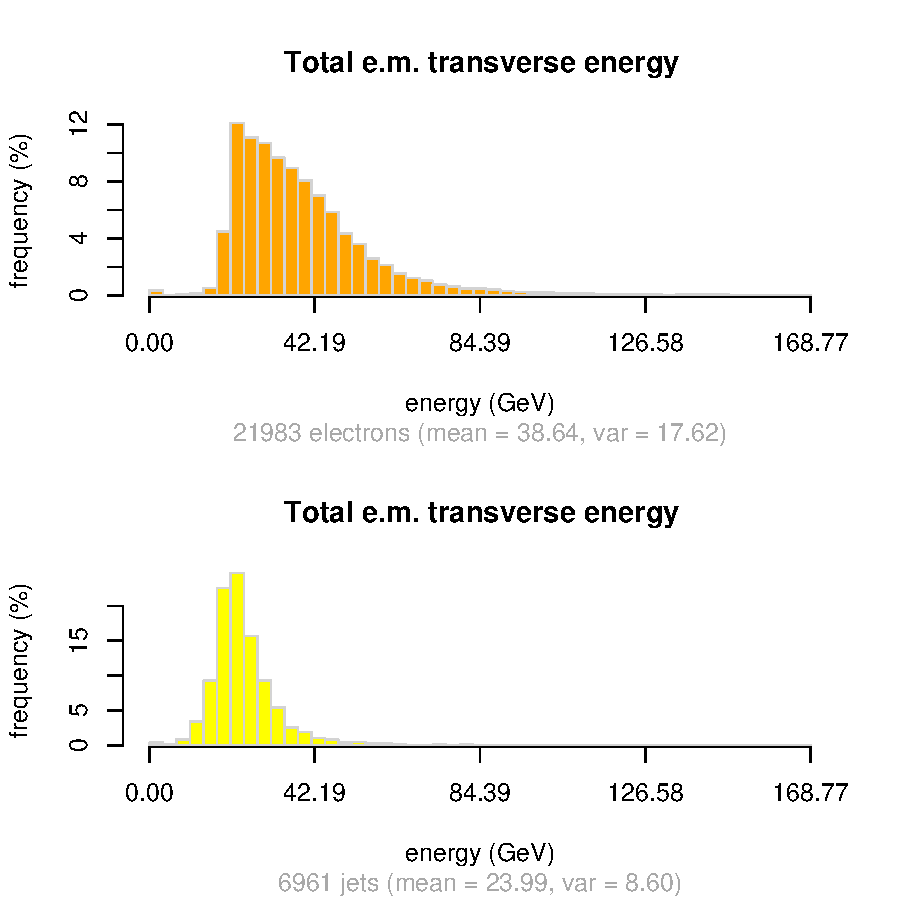
\includegraphics[scale=0.95]{em-tenergy}
\end{center}
\caption{A deposição total de energia na seção e.m. em uma região $0,4 \times
0,4$ no plano $\eta\times\phi$ para elétrons (em cima) e jatos (em baixo) para
a massa de dados disponível para o estudo. As contagens estão normalizadas.}
\label{fig:em-tenergy}
\end{figure}

\begin{figure}
\begin{center}
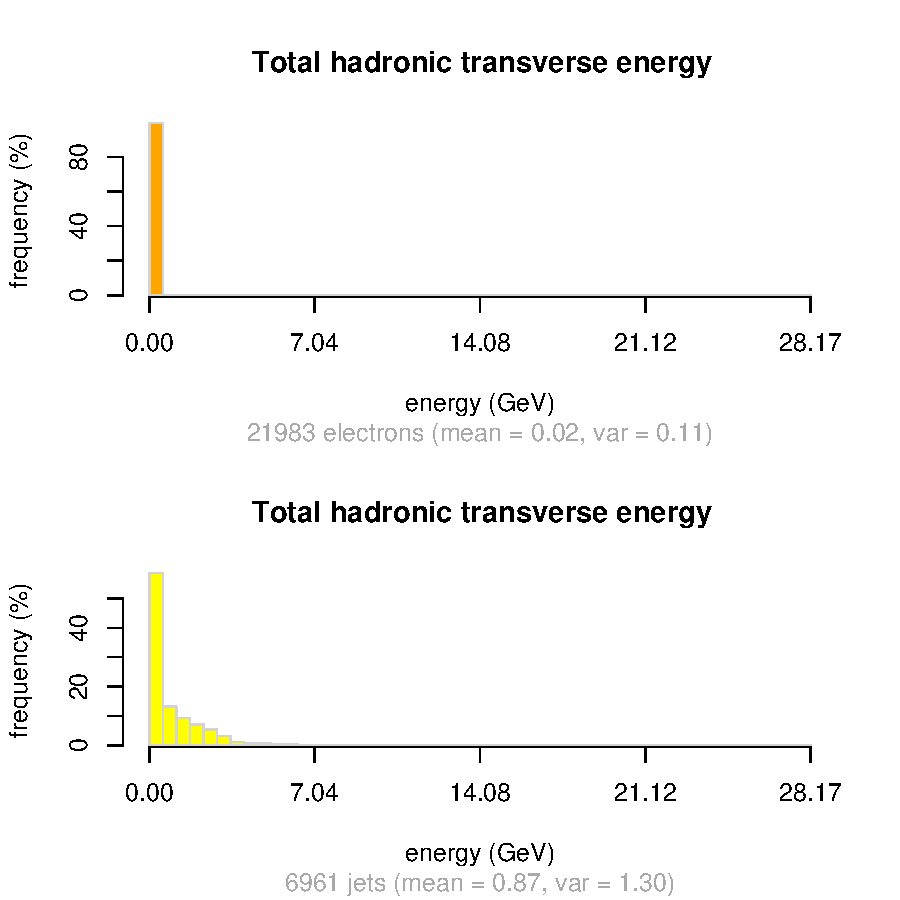
\includegraphics[scale=0.95]{had-tenergy}
\end{center}
\caption{A deposição total de energia na seção hadrônica em uma região $0,4 \times
0,4$ no plano $\eta\times\phi$ para elétrons (em cima) e jatos (em baixo) para
a massa de dados disponível para o estudo. As contagens estão normalizadas.}
\label{fig:had-tenergy}
\end{figure}

As Figuras~\ref{fig:rcore} e \ref{fig:eratio} mostram, respectivamente, a
fração \rcore e \eratio tal como utilizada pelo EGammaHypo para definir a
eficiência de deteção de elétrons e jatos. Na Figura~\ref{fig:rcore}
observa-se que a distribuição para elétrons tem média bastante próxima a 1 e
baixíssima variância. Para jatos a média é mais baixa e a distribuição
apresenta longa cauda em direção à origem. No caso da variável \eratio, que
tem por objetivo detetar picos de deposição energética na primeira camada
e.m., para elétrons observa-se um pico dominante em 1 ao passo que para jatos,
uma distribuição mais uniforme, indicando uma separabilidade linear.

\begin{figure}
\begin{center}
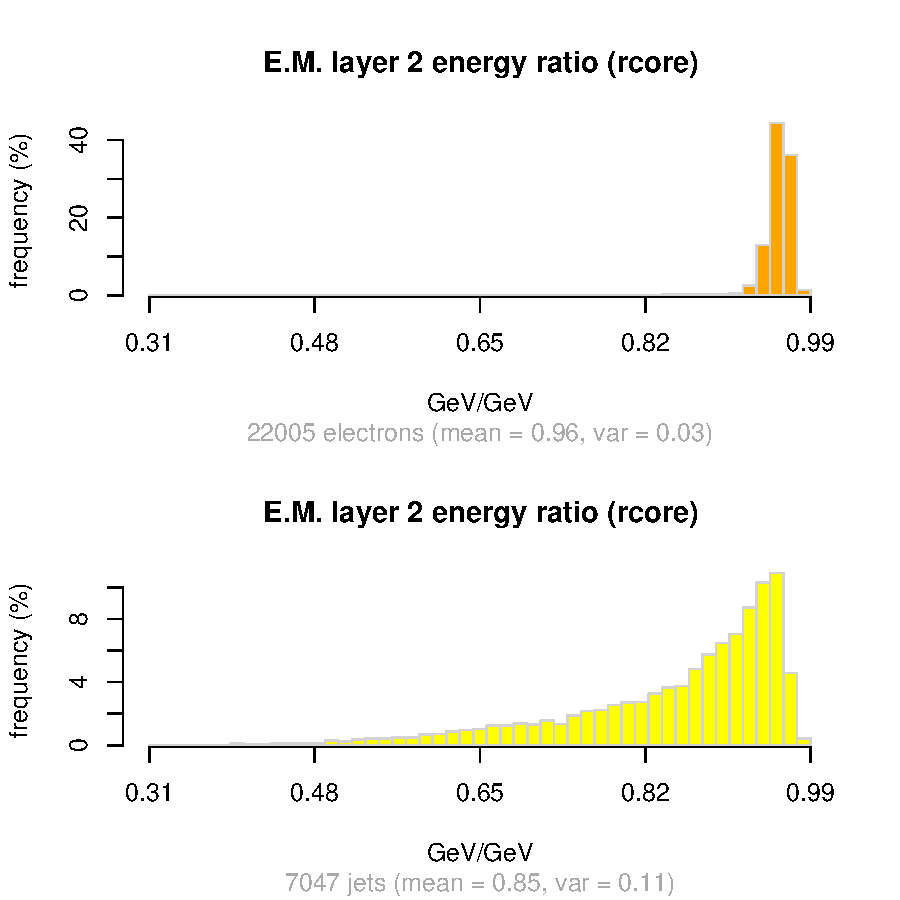
\includegraphics[scale=0.95]{rcore}
\end{center}
\caption{Distribuição da variável \rcore para elétrons (em cima) e jatos
(embaixo). As contagens estão normalizadas.}
\label{fig:rcore}
\end{figure}

\begin{figure}
\begin{center}
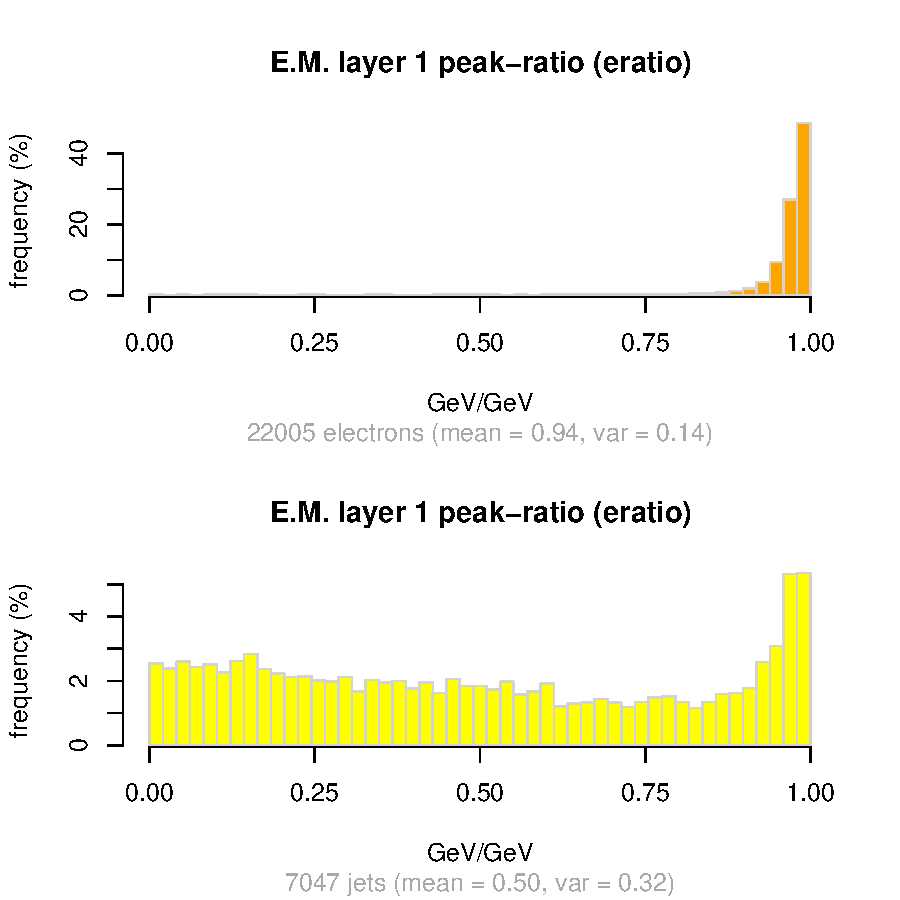
\includegraphics[scale=0.95]{eratio}
\end{center}
\caption{Distribuição da variável \eratio para elétrons (em cima) e jatos
(embaixo). As contagens estão normalizadas.}
\label{fig:eratio}
\end{figure}

As Figuras~\ref{fig:eta} e \ref{fig:phi} contém histogramas para elétrons (em
cima) e jatos (embaixo) dos centros refinados pelo T2Calo das RoI's em
questão, tanto em relação à variável $\eta$ quanto à variável $\phi$. É
possível distinguir uma uniformidade na distribuição em $\phi$ e uma tendência
a concentração de eventos nas proximidades de $\eta=0$, como é aguardado no
experimento.

\begin{figure}
\begin{center}
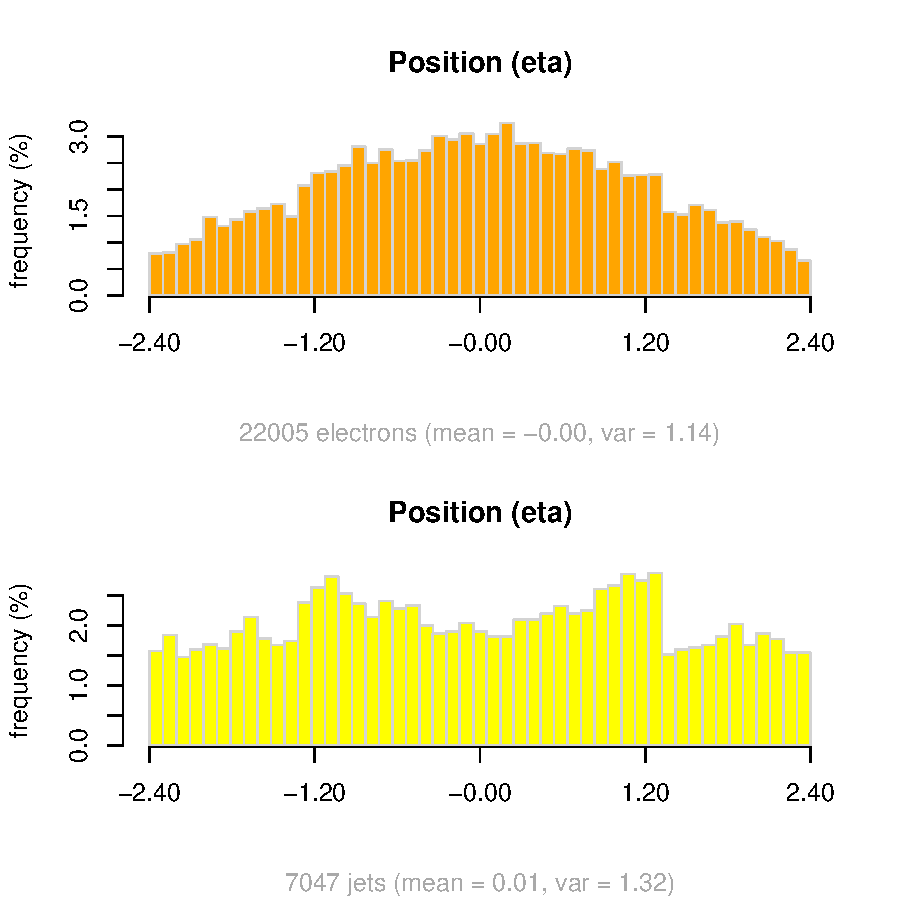
\includegraphics[scale=0.95]{eta}
\end{center}
\caption{Distribuição em $\eta$ dos centros refinados das RoI's para elétrons
(em cima) e jatos (embaixo). As contagens estão normalizadas.}
\label{fig:eta}
\end{figure}

\begin{figure}
\begin{center}
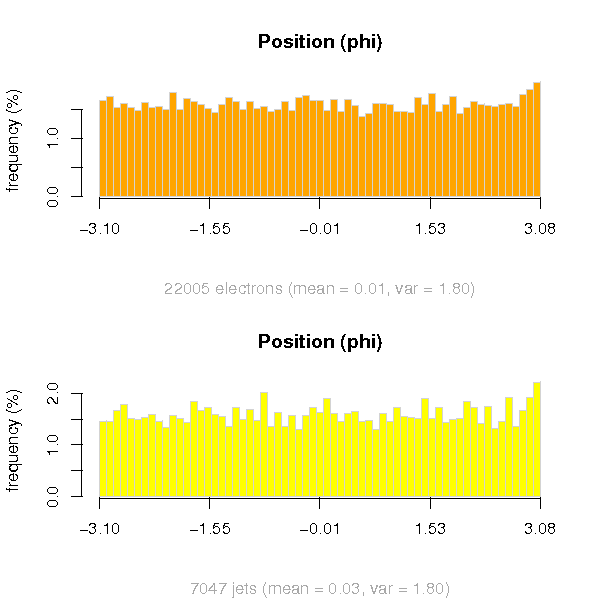
\includegraphics[scale=0.95]{phi}
\end{center}
\caption{Distribuição em $\phi$ dos centros refinados das RoI's para elétrons
(em cima) e jatos (embaixo). As contagens estão normalizadas.}
\label{fig:phi}
\end{figure}

Exceto por eventuais problemas na lógica de simulação (Monte Carlo) e
filtragem (pelo LVL1), estima-se que a massa de dados seja representativa do
problema da separação entre jatos e elétrons. Deve ser levado em consideração
que, para jatos, o pico ao redor de 25~GeV poderá introduzir imprecisões na
definição da capacidade de deteção de elétrons bastante energéticos, presentes
na massa de estudo. Sempre que possível, tentar-se-á levar estas restrições em
consideração.

\subsubsection{Deteção de elétrons com o EGammaHypo e sua otimização}
\label{sec:eghypo}

Para que a qualidade deteção do algoritmo proposto pelo EGammaHypo seja
estimada, deve-se passar a massa de dados de estudo por um processo de
otimização que ajude o especialista a selecionar os patamares de corte que
definem o algoritmo, como exposto na Seção~\ref{sec:classic-detection}. Para
tal, dividiu-se o conjunto de dados em 2 metades com aproximadamente o mesmo
número de RoI's. A primeira metade será utilizada para o ``treinamento'' ou
otimização dos cortes enquanto que a segunda será utilizada para o teste dos
cortes, garantindo a imparcialidade do processo.

O algoritmo de otimização não será exaustivo, varrendo todo o espaço de dados,
mas partirá de patamares pré-fixados em valores intuitivos e definirá uma
sub-área de variação por onde testará exaustivamente as combinações dos 4
cortes necessários, como é normalmente feito atualmente. Eis aqui os patamares
e passos de busca utilizados:

\begin{enumerate}
\item Corte em \rcore: de 0,6 a 1,0, em passos de 0,01 (41 possibilidades);
\item Corte em \eratio: de 0,6 a 1,0, em passos de 0,01 (41 possibilidades);
\item Corte em \etem: de 5000 a 30000 MeV em passos de 500 MeV (51
possibilidades);
\item Corte em \ethad: de 0 a 4000 MeV em passos de 500 MeV (9
possibilidades). 
\end{enumerate}

Para cada corte, a totalidade da massa de dados de treinamento do método é
avaliada e as RoI's que \textit{sobrevivam} ao corte são levadas à próxima
etapa. As eficiências relativas e a quantidade de dados utilizadas para o teste
da fase seguinte são acumulados para posterior análise. Levando-se em
consideração o número combinações dadas as possibilidades do problema de
otimização e considerando-se que a superfície de erro não possua um único
mínimo, há de se tentar $41 \times 41 \times 51 \times 9 = 771579$ diferentes
combinações, neste caso, antes de qualquer conclusão.

Esta claro que uma otimização não-polarizada estaria fora de questão para uma
utilização em condições que possam variar em questão de horas, como é o caso do
experimento ATLAS. Desta forma, seja uma antecipação para os cortes seria
necessária ou uma redução do espaço de busca permitindo uma otimização mais
rápida. A utilização de programas especialmente codificados para a tarefa
também poderia diminuir o tempo de teste, tornando o método mais atraente para
uma utilização prática.

A Figura~\ref{fig:eghypo-best-sp-train} mostra os resultados da busca
exaustiva definida anteriormente. Esta figura de mérito, normalmente
chamada de \textit{Característica Operacional do Receptor} (do inglês,
\eng{Receiver Operator Characteristics}, ROC \cite{vantrees}), contém os
resultados de cada ponto de operação do algoritmo EGammaHypo. O eixo vertical
denota a eficiência na deteção do sinal de interesse (elétrons), enquanto o
eixo horizontal, a taxa de falso-alarme (erro em jatos) naquele ponto de
operação. A taxa de falso alarme é escalonada em 25~kHz, que é a taxa de ruído
de fundo esperada, máxima. O valor do eixo horizontal portanto, denota a
quantidade de jatos que serão aprovados pelo LVL2, como elétrons e portanto
representa uma medida direta da taxa de eventos descarregados no Filtro de
Eventos.

Observa-se que, para o conjunto de intervalos testado, a massa de resultados
assume uma forma angulada. Ao redor do ponto de flexão, na parte exterior da
massa de resultados, encontraremos as melhores relações de eficiência
\textit{versus} falso-alarme para este discriminador. O ponto destacado nesta
figura representa o conjunto de cortes que maximiza a multiplicação da soma
eficiências de deteção pelo produto entre elas, ou seja:

\begin{equation}
SP = (\text{efic.}_{classe_1} + \text{efic.}_{classe_2}) \times (\text{efic.}_{classe_1} \times \text{efic.}_{classe_2})
\end{equation}

Este produto, de agora em diante chamado de produto SP, será usado como figura
de mérito, junto a curva ROC, para a determinação da qualidade discriminatória
dos algoritmos que serão estudados. Neste caso específico, o ponto onde
produto SP atinge seu máximo determina uma eficiência de deteção de elétrons
de 91,85 \% contra 10,19 \% de falso alarme na deteção de jatos, ou 2,55 kHz,
levando-se em consideração a contaminação do canal de elétrons na saída do
LVL1. O valor do produto SP no ponto em questão é de $1,50$.

\begin{figure}
\begin{center}
\includegraphics[scale=0.98]{eghypo/eghypo-best-sp-train.pdf}
\end{center}
\caption{A curva ROC para 771.579 combinações de valores de corte para o
algoritmo EGammaHypo.}
\label{fig:eghypo-best-sp-train}
\end{figure}

Os seguintes valores de corte determinam o detetor marcado na
Figura~\ref{fig:eghypo-best-sp-train}:
\begin{enumerate}
\item \rcore: 0.93;
\item \eratio: 0.82;
\item \etem: 14.500 MeV;
\item \ethad: 500 MeV.
\end{enumerate}

Aplicando-se estes cortes ao conjunto de treinamento, de forma análoga,
obtém-se 91,62 \% de eficiência na deteção de elétrons contra 10,45 \% de
falso-alarme ($SP = 1,49$). Este resultado indica também que os dois
sub-conjuntos de dados (treino e teste) são estatisticamente
semelhantes. Durante a busca exaustiva deste resultado, acumulou-se os
resultados de eficiência e falso-alarme parciais entre cada operação de
corte. Estes valores podem ser vistos na
Tabela~\ref{tab:eghypo-partials}. Como é possível avaliar à partir desta
tabela, as variáveis \rcore e \eratio são as mais discriminatórias, deixando
passar apenas cerca de 30 \% e 45 \% dos jatos avaliados, respectivamente. O
corte em \etem não reduz a taxa de eventos, sendo praticamente irrelevante ao
processo de discriminação. O vazamento de energia na seção hadrônica (último
corte), ainda conseguirá diminuir a taxa de falsos-positivos na saída do
detetor.

%% COMENTÁRIO: SERIA BOM DIZER PORQUE O CORTE EM EM_ET NÃO É TÃO RELEVANTE...
%% IDÉIAS: ALTA CORRELAÇÃO COM RCORE E ERATIO => PCA?

\begin{table}
\begin{center}
\begin{tabular}{|l|l|r|r|}
\hline
\textbf{Ordem} & \textbf{Variável} & \textbf{Eficiência (\%)} &
\textbf{Falso-alarme (\%)} \\ \hline
1 & \rcore & 96,4 & 30,5 \\ \hline
2 & \eratio & 95,7 & 43,6 \\ \hline
3 & \etem & 99,9 & \textbf{98,9} \\ \hline
4 & \ethad & 91.8 & 77.4 \\ \hline
\end{tabular}
\end{center}
\caption{Valores parciais de deteção e falso-alarme para o detetor baseado no
algoritmo EGammaHypo.}
\label{tab:eghypo-partials}
\end{table}

As Figuras~\ref{fig:eghypo-eta-scan-test}, \ref{fig:eghypo-phi-scan-test} e
\ref{fig:eghypo-emet-scan-test} contém os valores parciais de eficiência e
falso-alarme considerando-se uma divisão dos dados por $\eta$, $\phi$ e por
energia total transversa na seção e.m. dos calorímetros. No caso da varredura
em $\eta$, é possível notar que a eficiência de deteção do método apresenta
uma queda abrupta próximo ao vão entre a seção do barril e da tampa ($\eta
\approx 1,5$). Para a varredura em $\phi$, observa-se uma distribuição
bastante homogênea para a eficiência de deteção de elétrons e maior variação
na taxa de falso-alarme para jatos, possivelmente devido à baixa estatística
(muitos canais possuem apenas 30 a 40 jatos, como é possível observar na
Figura~\ref{fig:transverse-energy}). A varredura por \etem indica que o método
seja bastante robusto na deteção de elétrons, aumentando sua eficiência
suavemente com o valor de energia da RoI. O falso-alarme em jatos também
aumenta com a energia do objeto analisado, embora seja difícil estimar com
precisão a qualidade do valor de falso-alarme determinado, uma vez que a
estatística para jatos acima de 50 GeV seja praticamente inexistente.

\begin{figure}
\begin{center}
%\includegraphics[angle=90,width=15cm,height=20cm]{eghypo-eta-scan-test.pdf}
\includegraphics[scale=0.98]{eghypo/eghypo-eta-scan-test.pdf}
\end{center}
\caption{Eficiência de deteção (em preto) contra
falso-alarme (em cinza-claro/vermelho) por $\eta$.}
\label{fig:eghypo-eta-scan-test}
\end{figure}

\begin{figure}
\begin{center}
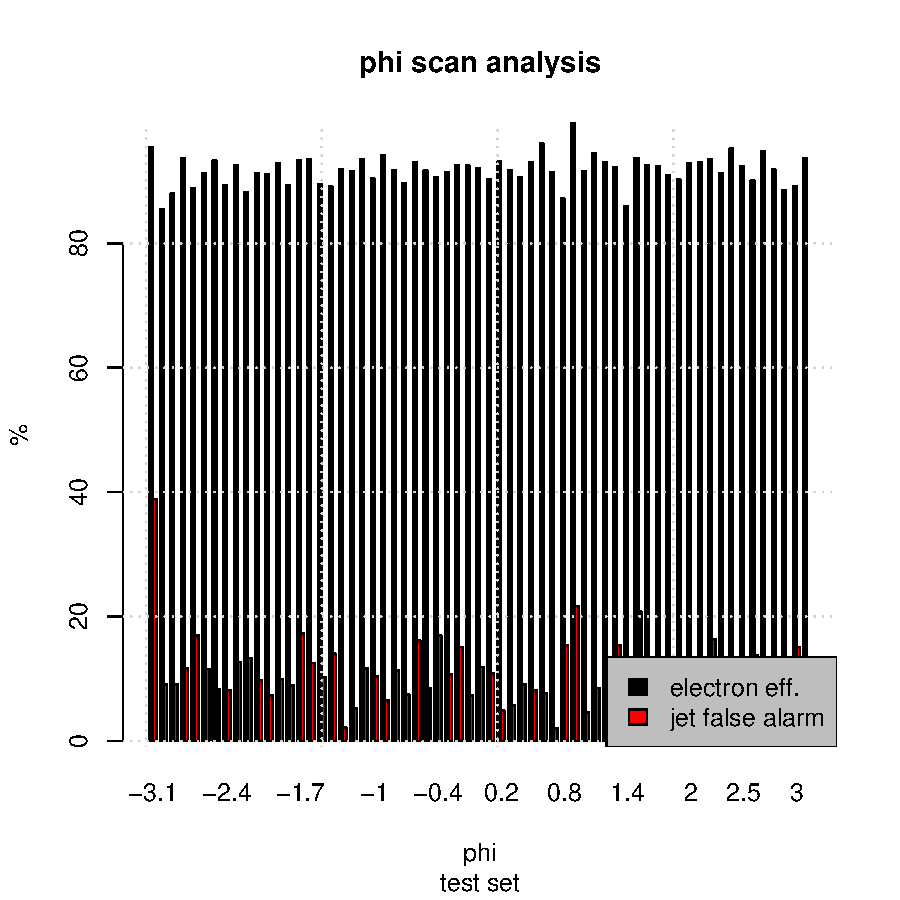
\includegraphics[scale=0.98]{eghypo/eghypo-phi-scan-test.pdf}
\end{center}
\caption{Eficiência de deteção (em preto) contra
falso-alarme (em cinza-claro/vermelho) por $\phi$.}
\label{fig:eghypo-phi-scan-test}
\end{figure}

\begin{figure}
\begin{center}
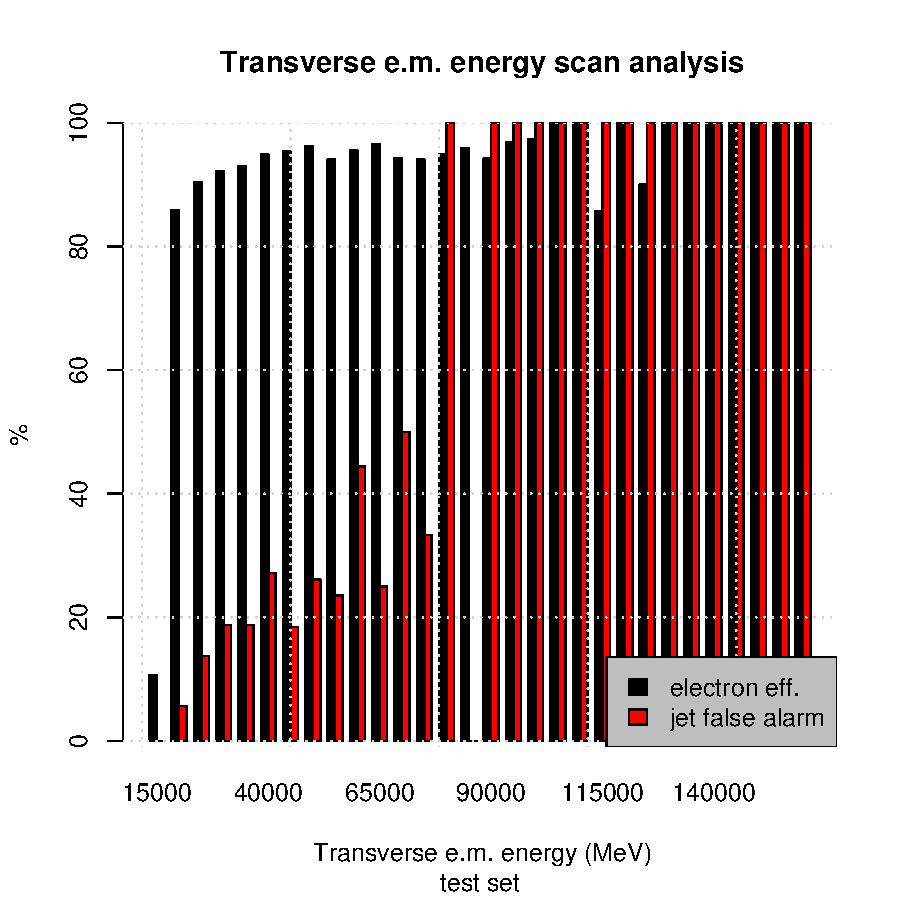
\includegraphics[scale=0.98]{eghypo/eghypo-emet-scan-test.pdf}
\end{center}
\caption{Eficiência de deteção (em preto) contra falso-alarme (em
cinza-claro/vermelho) por \etem.}
\label{fig:eghypo-emet-scan-test}
\end{figure}

%\subsubsection{Análise de Componentes Principais}

%Isto não é óbvio que melhorará a análise do método já que temos poucas
%variáveis a a informação contida nelas traz bastante informação, mas não
%informação discriminante.

%Levando-se em consideração os dados da Tabela~\ref{tab:eghypo-partials}, é
%possível intuir que exista uma grande correlação entre as 4 variáveis
%definidas pelo T2Calo e utilizados pelo EGammaHypo para a deteção de
%elétrons. A técnica de Análise de Componentes Principais \cite{vantrees}
%define uma transformação linear que, quando aplicada a massa de dados de onde
%é originalmente extraída, completamente a descorrelaciona. Esta transformada
%é comumente conhecida como KLT (do inglês \eng{Karhunen-Loève Transform}).

%Uma das técnicas para o cálculo da KLT utiliza a matriz de covariância C do
%conjunto de dados de analisados para calcular 

%\cite{vantrees}, é possível calcular a transformação , que
%completamente descorrelacionará os dados disponíveis. 

\section{Discriminação Linear}
\label{sec:lms}

O discriminador de Fisher \cite{fisher} ou a Análise de Discriminação Linear
\cite{duda} descrevem algoritmos bem definidos para que se maximize a
capacidade discriminante de um corte no plano com N dimensões, que separa duas
classes de amostras. Esta técnica requer que determinadas características nas
amostras estejam presentes, entre elas, que os dados apresentem uma
distribuição gaussiana e que as matrizes de covariância para ambas as classes
em separado sejam idênticas\footnote{A Análise de Discriminação Quadrática
\cite{duda}, no entanto, demonstra que esta característica pode ser relaxada
considerando-se que seja sempre possível projetar, através de uma
transformação linear, o espaço de entrada em um outro espaço onde as matrizes
de covariância sejam iguais e portanto recaindo no caso simples.}. Muitas
vezes, na prática, os valores de média e a covariância não estão disponíveis e
devem ser estimados, o que normalmente leva a falhas no cálculo do ponto ótimo
de discriminação. Dentre as técnicas de estimação da média e covariância
pode-se destacar a estimação por máxima verossimilhança ou por máximo a
\textit{posteriori}.

Em posse dos valores de média e covariância das classes, o plano de separação
seria definido da seguinte forma:

\begin{equation}
\overrightarrow{w} = \Sigma^{-1}(\overrightarrow{\mu}_0 -
\overrightarrow{\mu}_1) 
\end{equation}

Onde $\Sigma$ é a covariância ou \textit{variância cruzada} das observações do
universo de entrada e $\mu$ as médias das duas classes de eventos que se
deseja separar. Um problema que se segue é da invertibilidade de $\Sigma$, que
dependerá de quão bem o conjunto de amostras representa as classes a serem
discriminadas. Por exemplo, se $\Sigma$ possui combinações lineares dos dados
disponíveis, o ranque desta matriz será inferior ao número de amostras e
portanto a matriz não será invertível. Embora existam técnicas para superar o
problema, é possível fazer uso de outras técnicas derivadas deste sistema
primário para maximizarmos a discriminação das classes dado um conjunto de
amostras.

Por causa das dificuldades discutidas, muitas técnicas iterativas surgiram
para que seja possível a definição de um plano ótimo de separação linear à
partir de amostras de dados reais. Dentre elas, o algoritmo do Mínimo Médio
Quadrático \cite{widrow} (do inglês \eng{Least Mean Square} ou LMS) está
dentre os mais utilizados. Este método pode ser considerado um caso especial
de uma rede neural totalmente conectada e sem realimentação (veja
Seção~\ref{sec:neural} para uma discussão mais detalhada), com as seguintes
ressalvas:

\begin{itemize}
\item Há somente um neurônio conectando todas as entradas com a saída da rede;
\item A função de ativação deste neurônio ($\phi(\dot)$) é a função identidade
$f(x) = x$.
\end{itemize}

Para o treinamento, define-se alvos para as duas classes de eventos e a função
de erro:

\begin{equation}
E(\overrightarrow{w}) = \frac{1}{2} e^2(n)
\end{equation}

Onde $\overrightarrow{w}$ é o vetor de pesos que define o plano de separação
linear e $e(n)$ é o erro na saída da rede com relação ao alvo para a classe
escolhida com relação a amostra $n$, ou seja $e(n) = d(n)-y(n)$ ($d(n)$ é o
alvo). Desta forma, derivando-se esta função de erro com relação aos pesos
sinápticos $\overrightarrow{w}$, mostra-se que o gradiente de $E$ será:

\begin{equation}
\frac{\partial E(\overrightarrow{w})}{\partial \overrightarrow{w}} =
-x(n)e(n) 
\end{equation}

Onde $x(n)$ é a n-ésima entrada que leva o neurônio linear a uma saída
$y(n)$. E, com este resultado, define-se a fórmula de treinamento do LMS:

\begin{equation}
\hat{w}(n+1) = \hat{w}(n) + \alpha x(n)e(n)
\label{eq:lms}
\end{equation}

Onde $\alpha$ representa a taxa de aprendizagem, um parâmetro para a suavização
da trajetória do treinamento no espaço da função de erro
$E(\overrightarrow{w})$. A Equação~\ref{eq:lms} representa a fórmula clássica
do treinamento de um classificador LMS, indicando um método bem-definido de
atualização dos pesos da rede para que se convirja a um erro mínimo. Na
prática, é possível ainda definir técnicas de treinamento em bateladas para se
obter uma suavização do treinamento em direção ao mínimo global, ainda que
garantido devido à superfície bem-definida do erro (quadrático). No
treinamento em bateladas ou épocas, os pesos sinápticos são corrigidos 
tendo por base a média dos erros para todos os eventos de uma época, ao invés
de individualmente. 

Para eliminar polarizações no processo de treinamento devido a magnitude das
componentes da entrada, enquanto comparadas entre si, é também prática que
cada entrada seja subtraída da sua média e dividida pela sua variância. A
Figura~\ref{fig:lms-flow} mostra o diagrama de blocos do discriminador LMS que
será empregado neste estudo. O valor da saída $y$ é utilizado para definir a
R.O.C. do discriminador e escolher, ao invés de quatro, apenas um corte que
maximize a capacidade discriminante do sistema. Alvos para cada uma das
classes são escolhidos e o sinal de erro é utilizado para corrigir os pesos
sinápticos, até que o sistema convirja para o erro mínimo.

\begin{figure}
\begin{center}
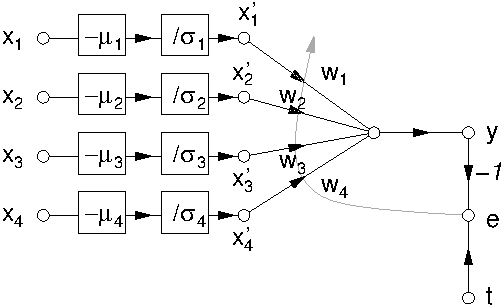
\includegraphics{lms-flow}
\end{center}
\caption{O diagrama de fluxo do discriminador LMS que será empregado na
discriminação elétron-jato.}
\label{fig:lms-flow}
\end{figure}

\subsection{Implementação do LMS na separação e\-lé\-tron-jato}
\label{sec:lms-ej}

Levando-se em consideração as 4 variáveis definidas pelo T2Calo, é possível
encontrar o plano quadri-dimensional que define um discriminador linear ótimo,
usando-se o algoritmo LMS, como descrito anteriormente. A separação em classes
de treinamento e teste como apresentada na Seção~\ref{sec:eghypo} será
re-aproveitada aqui, para seja possível a comparação dos resultados nos dois
casos.

O sistema de treinamento e teste foi implementado em um ambiente de trabalho
C++, seguindo o paradigma da orientação à objetos (OO). Este ambiente, que
será re-utilizado em várias partes deste trabalho, será discutido em detalhes
na Seção~\ref{sec:framework}. A Figura~\ref{fig:train-flow} contém um diagrama
de fluxo com os diversos passos do sistema de treinamento
implementando. Inicialmente, os bancos de dados usados para o treinamento e
teste da rede são carregados. Os valores de média e variância dos dados são
extraídos do conjunto de treinamento e guardados juntos aos pesos
$\hat{w}(n)$, para que sejam aplicados durante o treinamento\footnote{De fato,
seria mais eficiente que os fatores de normalização fossem aplicados
previamente ao treinamento. No entanto, uma vez que deseja-se re-aproveitar a
base de código para rodar o discriminador em uma etapa seguinte, é mais
simples do ponto de vista da implementação que a normalização seja aplicada
como parte do passo de execução do discriminador.}. Os pesos sinápticos são
aleatoriamente inicializados (entre $-1$ e $+1$. Valores-alvo para cada uma
das classes são pré-fixados: $-1$ para elétrons e $+1$ para jatos. O processo
de treinamento é então disparado. Para cada época ou batelada de treinamento,
um conjunto de elétrons e jatos é escolhido aleatoriamente à partir dos
bancos-de-dados disponíveis. Os valores de erro são calculados e sua média é
aplicada para a correção dos pesos sinápticos considerando a taxa de
aprendizagem $\alpha$. As melhores redes, tomando-se o valor do produto SP
como referência, são guardadas a cada passo de treinamento. Um sistema
configurável é utilizado para detetar a estagnação do treinamento. Quando o
sistema atinge um estado no qual as alterações sinápticas não modifiquem
significativamente o valor do produto SP do discriminador (levando-se em
consideração uma margem de erro) por um número de iterações, o treinamento é
automaticamente parado. O melhor discriminador até então é recarregado. Um
estudo dos valores de Erro Médio Quadrático (EMQ, do inglês \eng{Mean-square
error}, MSE) e produto SP é conduzido levando-se em consideração o corte que
maximiza o valor do produto SP para a rede considerando-se a massa de dados
disponível para teste.

\begin{figure}
\begin{center}
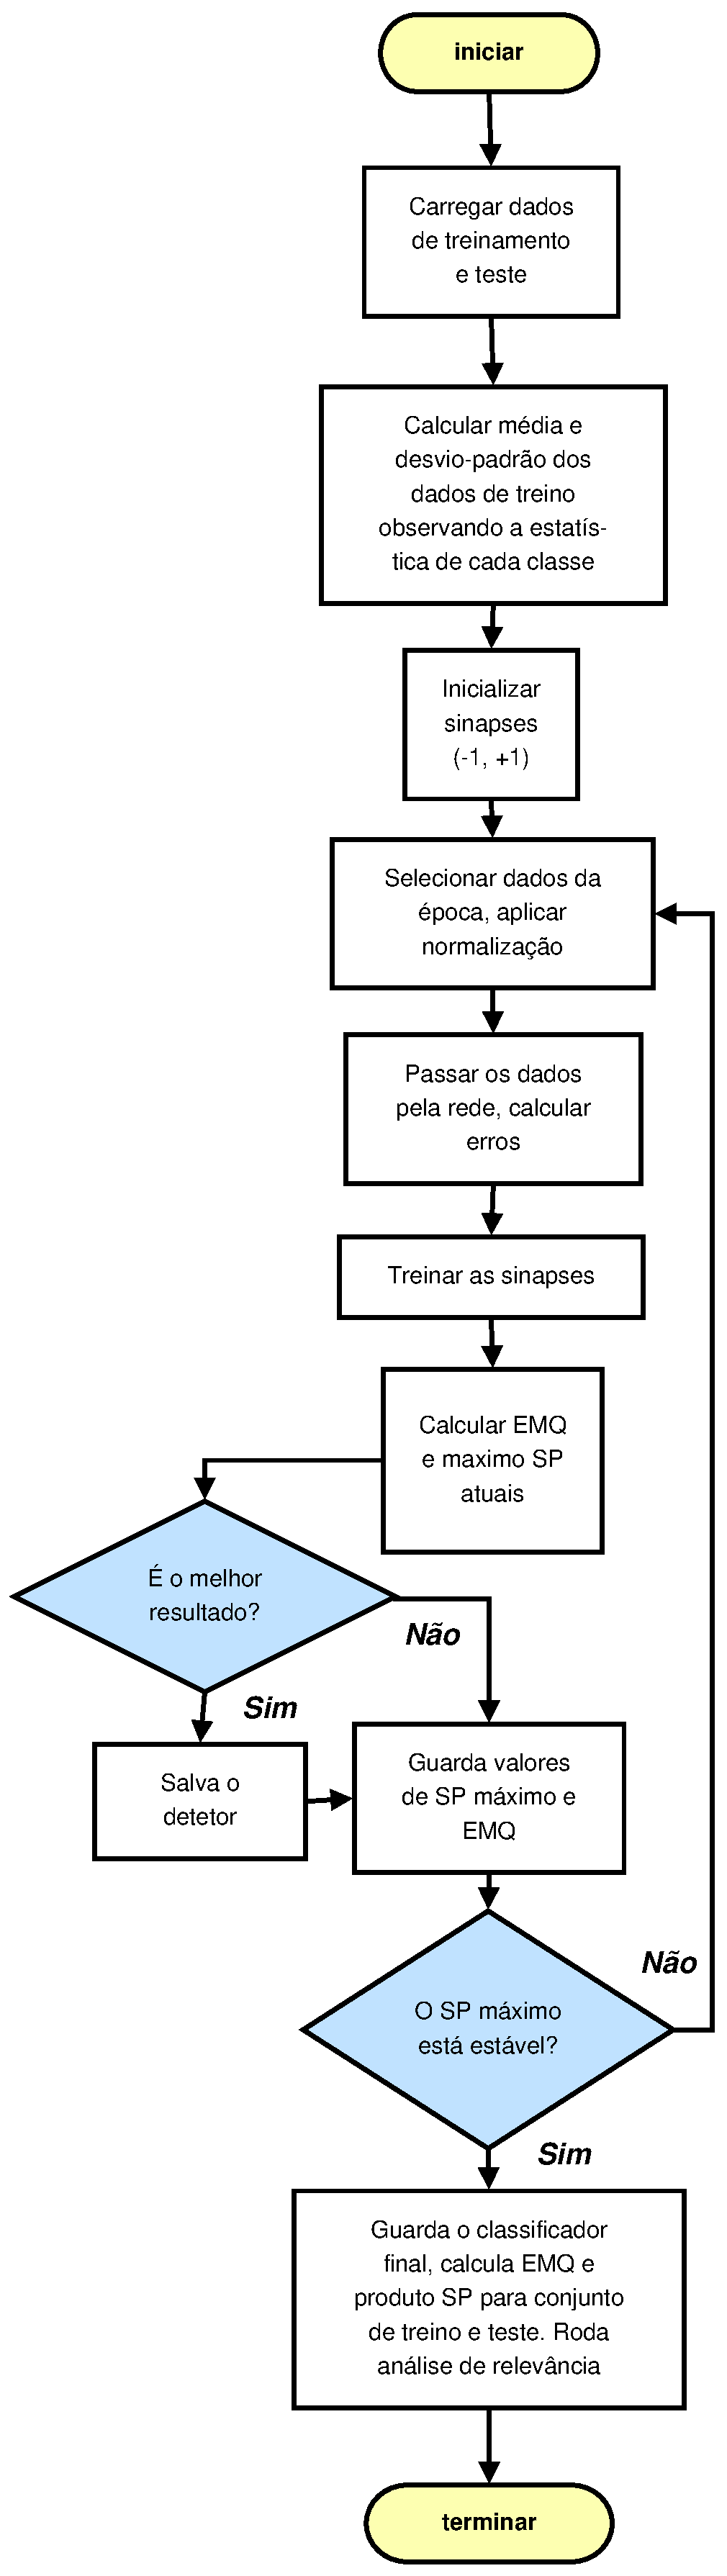
\includegraphics[scale=0.35]{train-flow}
\end{center}
\caption{O fluxo implementado para o treinamento do discriminador LMS.}
\label{fig:train-flow}
\end{figure}

\subsection{Resultados da aplicação do LMS na separação e\-lé\-tron-jato}

Utilizando o sistema descrito anteriormente, e a separação dos dados (em
classes de treinamento e teste) proposta no início do estudo, realizou-se um
conjunto de testes para a determinação de um discriminador linear ótimo
baseado nas variáveis extraídas pelo T2Calo. Dois parâmetros foram
considerados neste exercício:

\begin{itemize}
\item O número de elementos na batelada ($N$);
\item O valor da taxa de treinamento ($\alpha$).
\end{itemize}

Embora seja possível assumir que o sistema convergirá em todas as condições,
valores muito grandes para a taxa de treinamento (ou pequenos para a
quantidade de eventos na batelada) poderão fazer o processo de convergência ao
mínimo parecer instável e disparar erros no sistema de parada automática do
treinamento. Desta forma, conduziu-se um conjunto de testes para a
determinação dos parâmetros de treinamento que acarretem em uma migração suave
ao erro mínimo do discriminador, no menor tempo possível. Os resultados podem
ser vistos nas Figuras~\ref{fig:lms-lr-analysis} e
\ref{fig:lms-esize-analysis}. Cada ponto nestas figuras representa a média
sobre dez treinamentos realizados à partir de um conjunto de pesos iniciais
sorteados (uniformemente) aleatoriamente no intervalo $[-1, +1]$. Como é
possível observar através das figuras, para o problema em questão, o sistema
responde melhor a baixos valores de taxa de treinamento e valores
intermediários para o tamanho da batelada. Durante o experimento, limitou-se o
número máximo de passos de treinamento em $1.000$, de forma que instabilidades
durante o processo de convergência não impedissem o final da fase de
treinamento. Desta forma, pontos nas curvas próximos a este valor no eixo
vertical indicam provável instabilidade e que o treinamento foi interrompido
bruscamente pelo programa ao invés de convergir suavemente a um mínimo.

\begin{figure}
\begin{center}
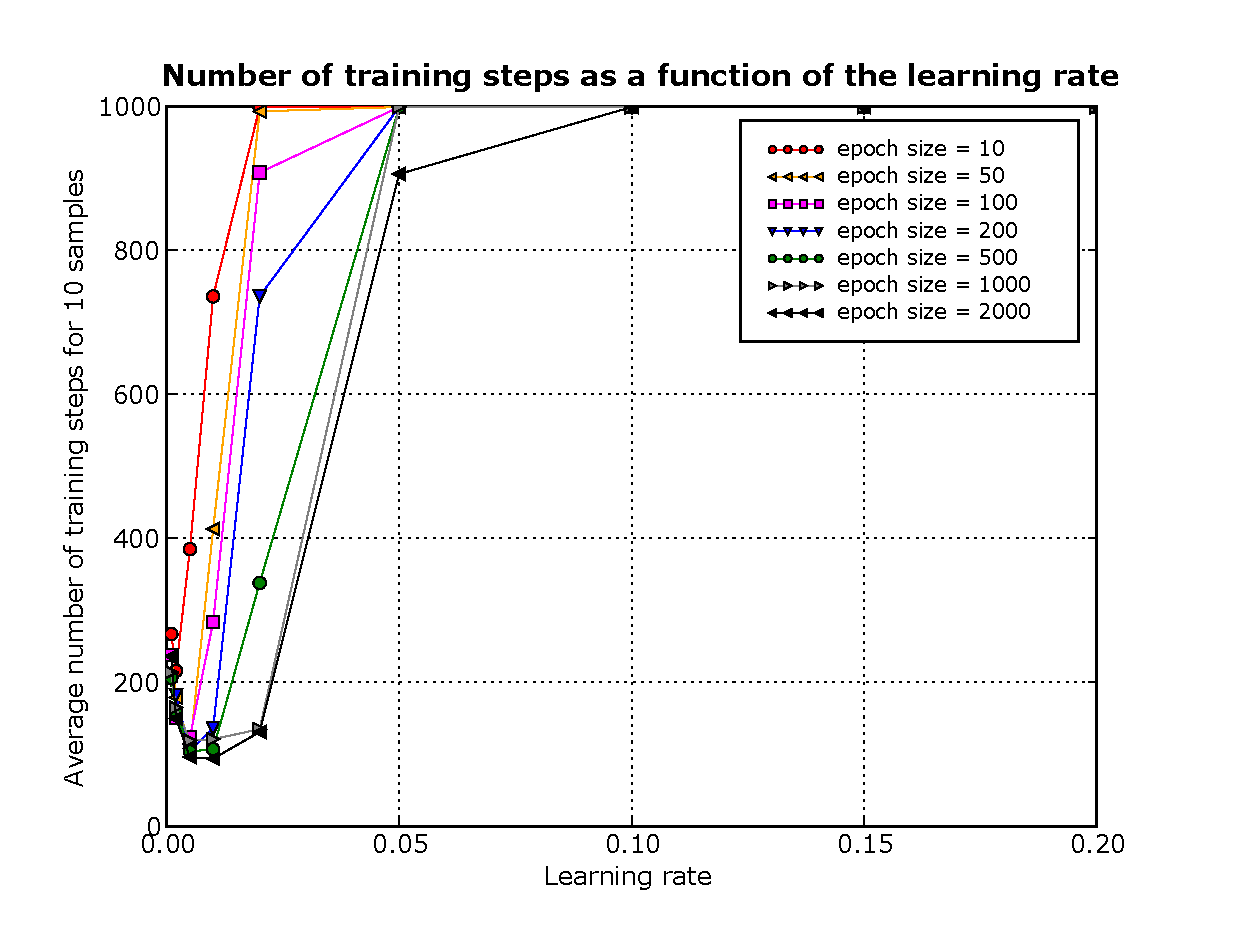
\includegraphics[scale=0.5]{lms/lms-lr-analysis}
\end{center}
\caption{Número de passos de treinamento médio (para 10 tentativas) em função
da taxa de treinamento para a discriminação elétron/jato.}
\label{fig:lms-lr-analysis}
\end{figure}

\begin{figure}
\begin{center}
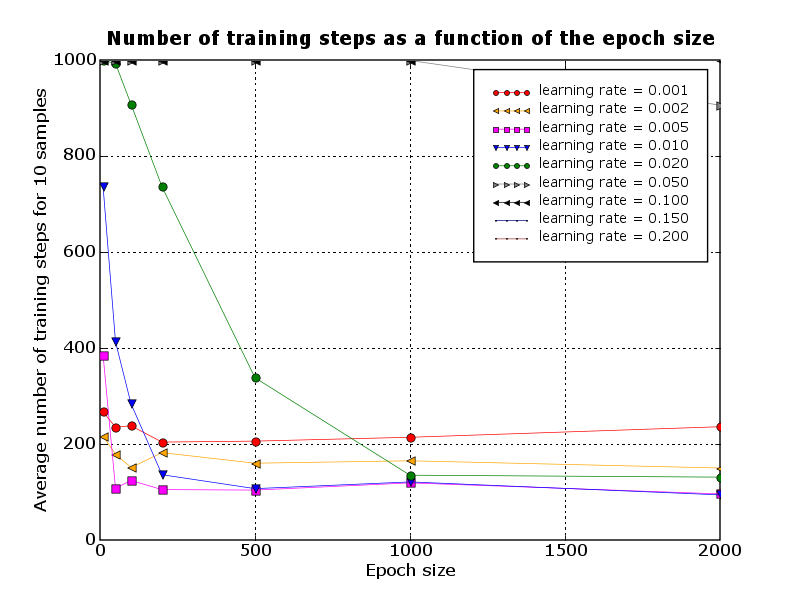
\includegraphics[scale=0.5]{lms/lms-esize-analysis}
\end{center}
\caption{Número de passos de treinamento médio (para 10 tentativas) em função
do tamanho da época para a discriminação elétron/jato.}
\label{fig:lms-esize-analysis}
\end{figure}

Uma análise visual nestes gráficos indicam que valores de taxa de treinamento
aconselháveis estão na faixa $\alpha < 0.02$, enquanto que um tamanho da época
favorável pareça ser $N > 200$. Escolhe-se $N = 500$ e $\alpha = 0.01$. Desta
forma, depois de cerca de 10 passos, cerca de 35\% do conjunto de treinamento
já foi usado. Com 30 a 40 passos, a rede já terá ``visto'' todos os dados de
treinamento ao menos uma vez, em média\footnote{O sorteio dos eventos de uma
batelada é feito de forma aleatória (distribuição uniforme) e não há garantias
que todos os eventos sejam utilizados ao longo do treinamento, embora seja
estatisticamente provável que isto aconteça.}.

A Figura~\ref{fig:lms-mse-evo} mostra a evolução do EMQ para uma das 10 redes
com $N = 500$ e $\eta = 0.01$, tanto para o conjunto de treinamento (no alto)
quanto para o conjunto de teste (embaixo). A Figura~\ref{fig:lms-sp-evo}
mostra um gráfico equivalente, mas para o produto SP ao invés do EMQ. Como é
possível verificar, o sistema converge depois de um pouco menos que 100 passos
de treinamento. A evolução do produto SP é compatível com a minimização do EMQ,
aumentando rapidamente no início do treinamento, por cerca de 20 passos e
depois permanecendo constante, em aproximadamente 1,5 para o restante do
treinamento. O mesmo não ocorre para o EMQ que ainda continuará a diminuir,
significativamente, por mais 60 a 80 passos antes da deteção automática da
parada. O perfil de evolução do produto SP e minimização do EMQ é seguido pelo
conjunto de teste, de forma bastante semelhante, indicando mais uma vez forte
semelhança estatística entre os dois grupos de dados.

\begin{figure}
\begin{center}
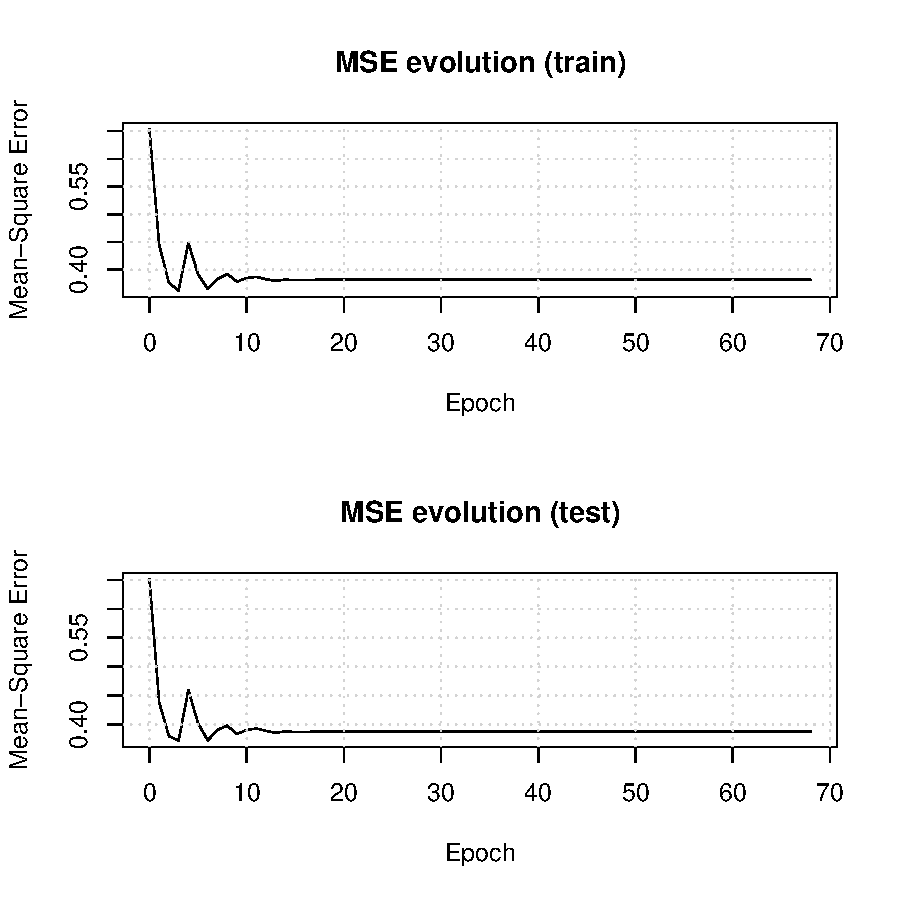
\includegraphics[scale=0.98]{lms/mse-evolution}
\end{center}
\caption{Evolução dos valores do E.M.Q. ao longo do treinamento, para o
conjunto de treinamento (topo) e de teste (embaixo).}
\label{fig:lms-mse-evo}
\end{figure}

\begin{figure}
\begin{center}
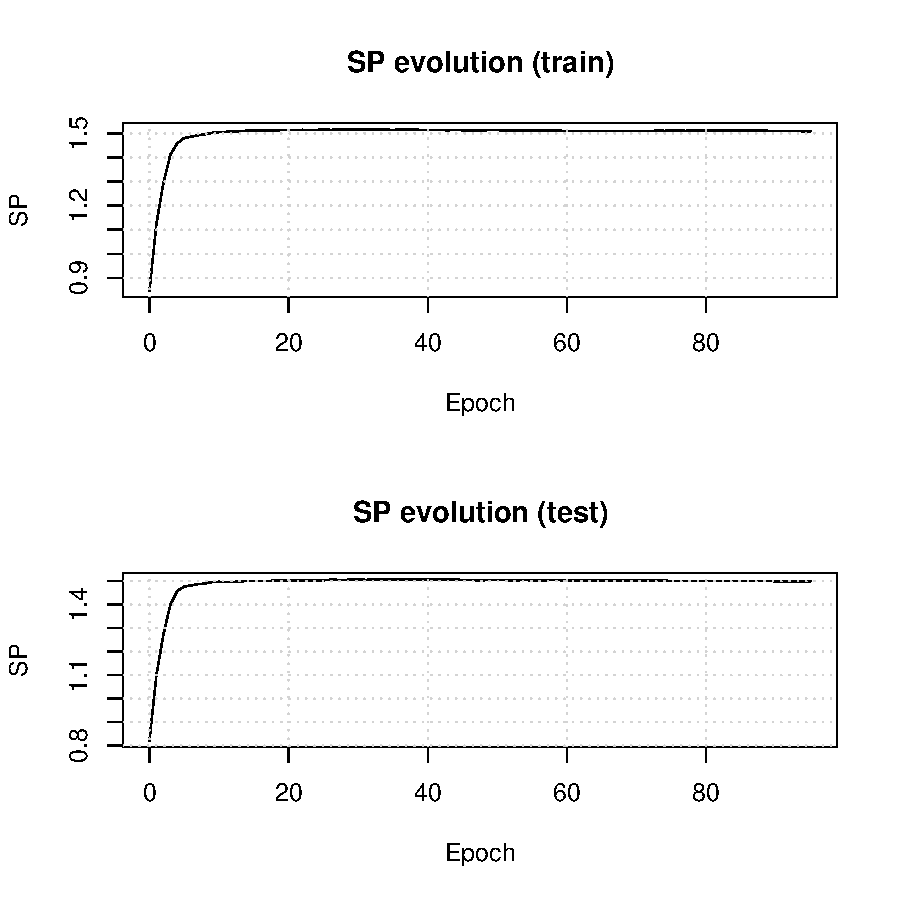
\includegraphics[scale=0.98]{lms/sp-evolution}
\end{center}
\caption{Evolução dos valores do produto SP ao longo do treinamento, para o
conjunto de treinamento (topo) e de teste (embaixo).}
\label{fig:lms-sp-evo}
\end{figure}

A Figura~\ref{fig:lms-test-output} contém os histogramas da saída da rede para
elétrons (alto) e jatos (embaixo), considerando-se o conjunto de teste. O
ponto ótimo de corte, determinado para que se maximize o produto SP da rede
para o conjunto de treinamento para este sistema é $-0,0473$. Nestas
condições, o máximo produto SP para o conjunto de teste é 1.51, definido no
ponto da curva R.O.C. (veja Figura~\ref{fig:lms-test-roc}) onde a eficiência
para a deteção de elétrons é 91,64\% enquanto que a eficiência para a deteção
de jatos é de 90,35\%. A Figura~\ref{fig:lms-vs-egamma-roc} mostra uma
comparativo entre o resultado da otimização proposta atualmente no experimento
ATLAS contra os resultados obtidos para este classificador. Através desta
figura é possível observar que o discriminador LMS tangencia a parte exterior
dos pontos da otimização proposta atualmente no experimento. O resultado
obtido com o algoritmo LMS, ao invés do longo processo de otimização proposto
originalmente, é atingido depois de apenas 1 minuto e 30 segundos de
treinamento, embora já apresente uma capacidade discriminatória praticamente
ótima após apenas 20 passos de treinamentos ($\approx 25$ segundos).

\begin{figure}
\begin{center}
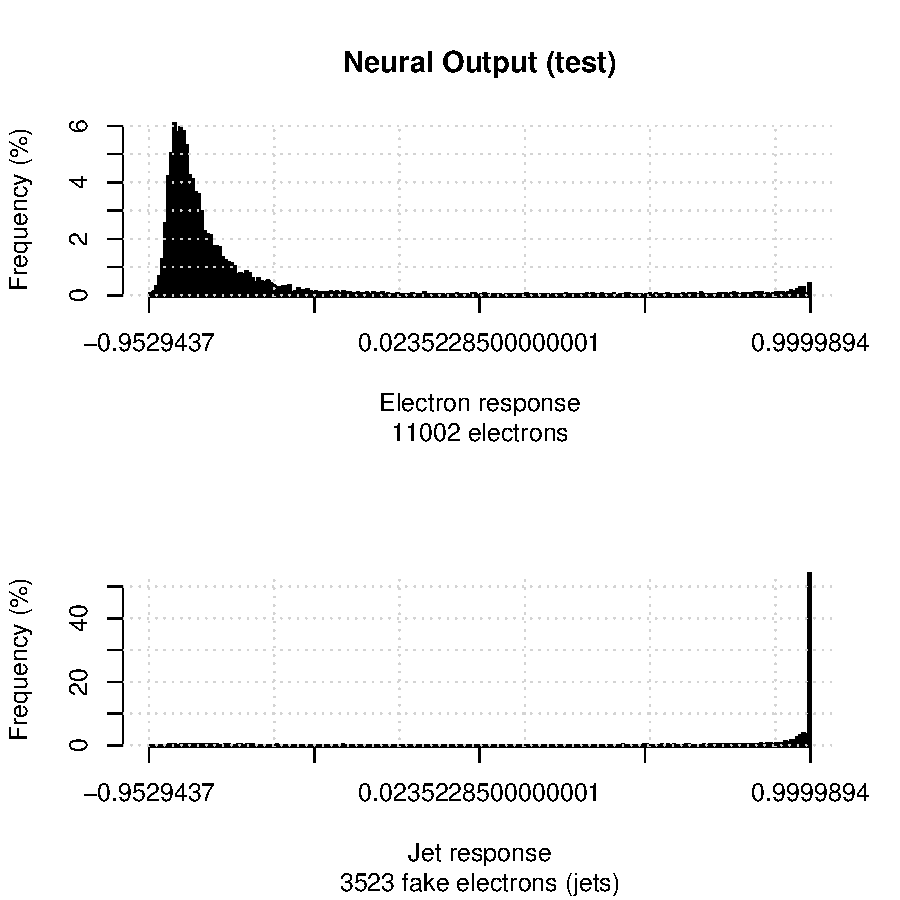
\includegraphics[scale=0.98]{lms/test-output}
\end{center}
\caption{Saída do detetor LMS para o conjunto de treino.}
\label{fig:lms-test-output}
\end{figure}

\begin{figure}
\begin{center}
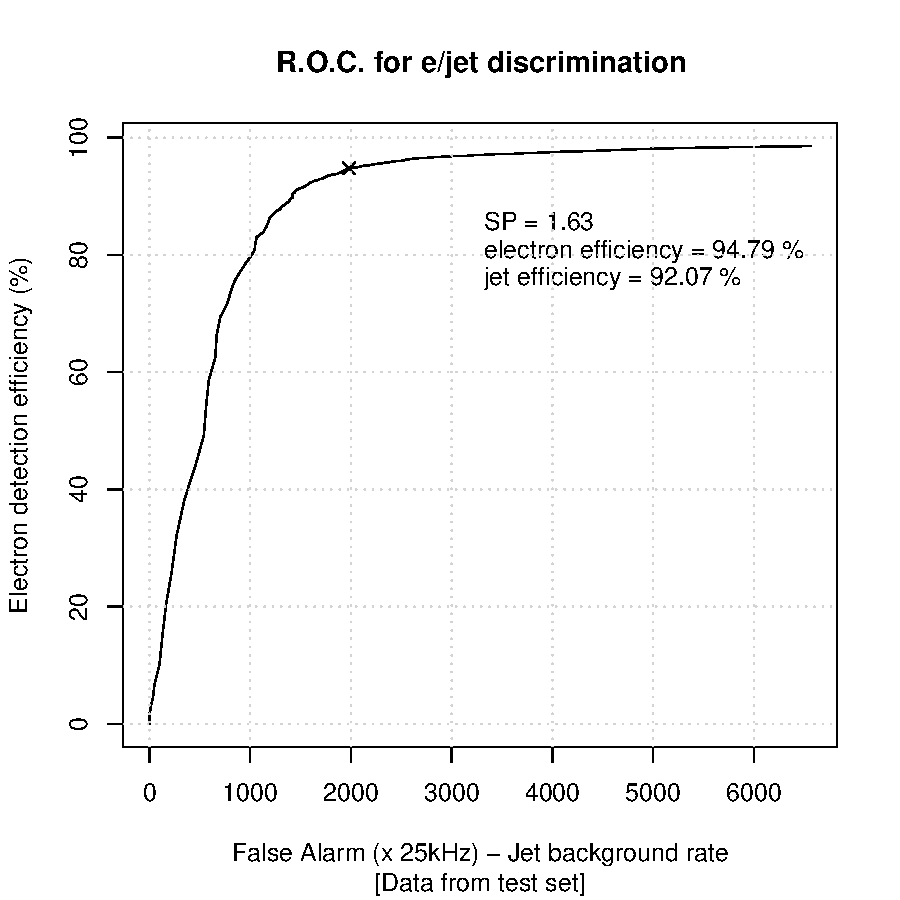
\includegraphics[scale=0.98]{lms/test-roc}
\end{center}
\caption{Curva R.O.C. para um detetor elétron/jato baseado no algoritmo LMS.}
\label{fig:lms-test-roc}
\end{figure}

\begin{figure}
\begin{center}
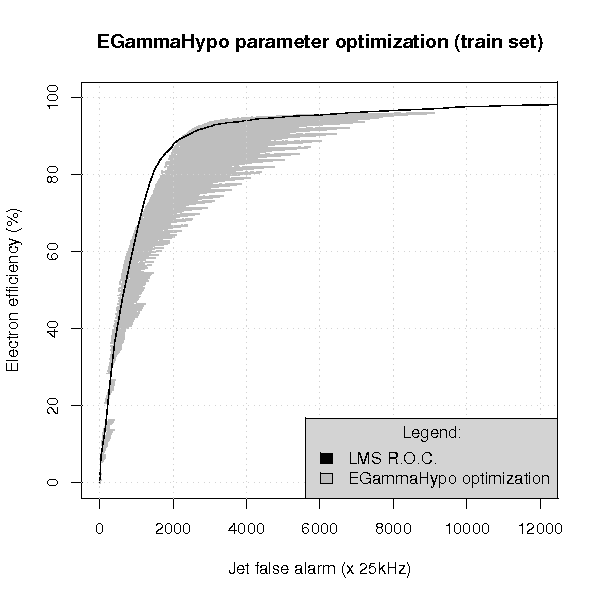
\includegraphics[scale=0.98]{lms/lms-vs-egamma-roc}
\end{center}
\caption{R.O.Cs comparativas entre a otimização atual para o EGammaHypo e um
detetor baseado no LMS.}
\label{fig:lms-vs-egamma-roc}
\end{figure}

As Figuras~\ref{fig:lms-test-sp-eta}, \ref{fig:lms-test-sp-phi} e
\ref{fig:lms-test-sp-emet} mostram, respectivamente, o valor do produto SP segundo
a distribuição dos dados em $\eta$, $\phi$ e $\etem$. O número anexo ao topo
de cada barra indica a quantidade de eventos dentro do limite em questão e é
útil para que se considere a relevância de um valor parcial no desempenho do
discriminador. Nota-se que na distribuição por $\eta$, há uma clara perda de
eficiência na região onde $|\eta| \approx 1,5$. Esta notável queda no
desempenho do classificador é devido a um espaço sem elementos de deteção
nesta área (também conhecido como \eng{gap} ou \eng{crack} dos calorímetros),
por onde passam os cabos de leitura e manutenção dos detetores internos. A
eficiência é recuperada logo após esta região e recai suavemente nas bordas. O
gráfico de barras para a distribuição $\phi$ mostra-se corretamente uniforme,
indicando que o sistema não está polarizado e funciona coerentemente para
todos os valores desta variável. Este resultado é esperado já que o detetor é
simétrico neste eixo. A análise por $\etem$ demonstra uma predominante
qualidade de deteção para valores mais baixos de energia que valores mais
altos. Deve-se levar em conta que, embora a eficiência de deteção de elétrons
ainda seja máxima nesta última região, como mostra a
Figura~\ref{fig:lms-test-efficiency-emet}, o falso alarme na deteção de jatos
também apresenta-se máximo. Uma vez que o produto SP é uma figura de mérito da
eficiência agregada de ambas as classes de eventos do discriminador, ela
quantificar-se-á em zero nesta região, o que é razoável. Este resultado está
notavelmente associado a baixa estatística disponível na região.

\begin{figure}
\begin{center}
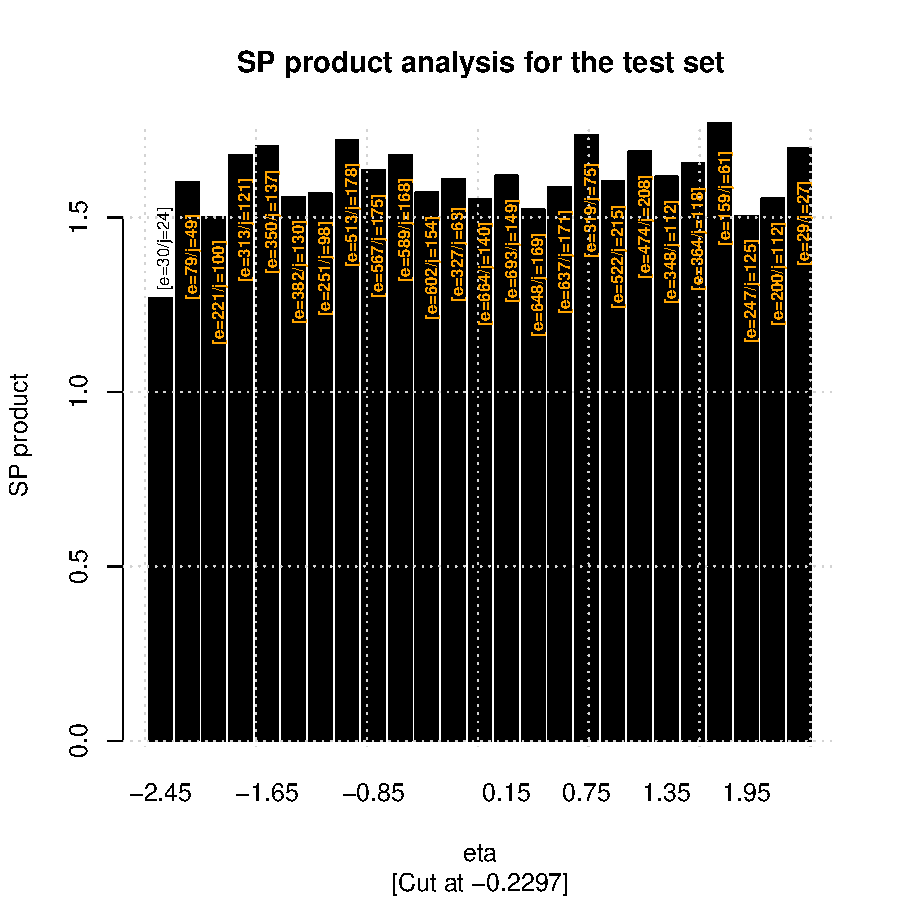
\includegraphics[scale=0.98]{lms/test-sp-eta}
\end{center}
\caption{Análise do produto SP ao longo de $\eta$.}
\label{fig:lms-test-sp-eta}
\end{figure}

\begin{figure}
\begin{center}
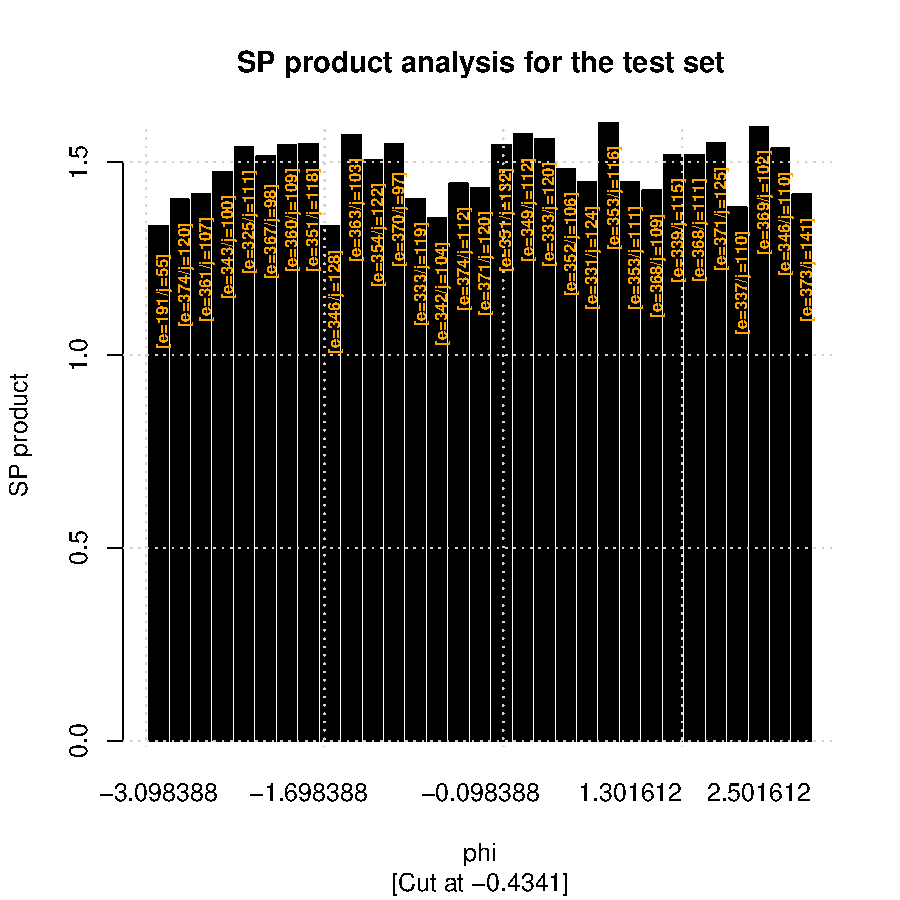
\includegraphics[scale=0.98]{lms/test-sp-phi}
\end{center}
\caption{Análise do produto SP ao longo de $\phi$.}
\label{fig:lms-test-sp-phi}
\end{figure}

\begin{figure}
\begin{center}
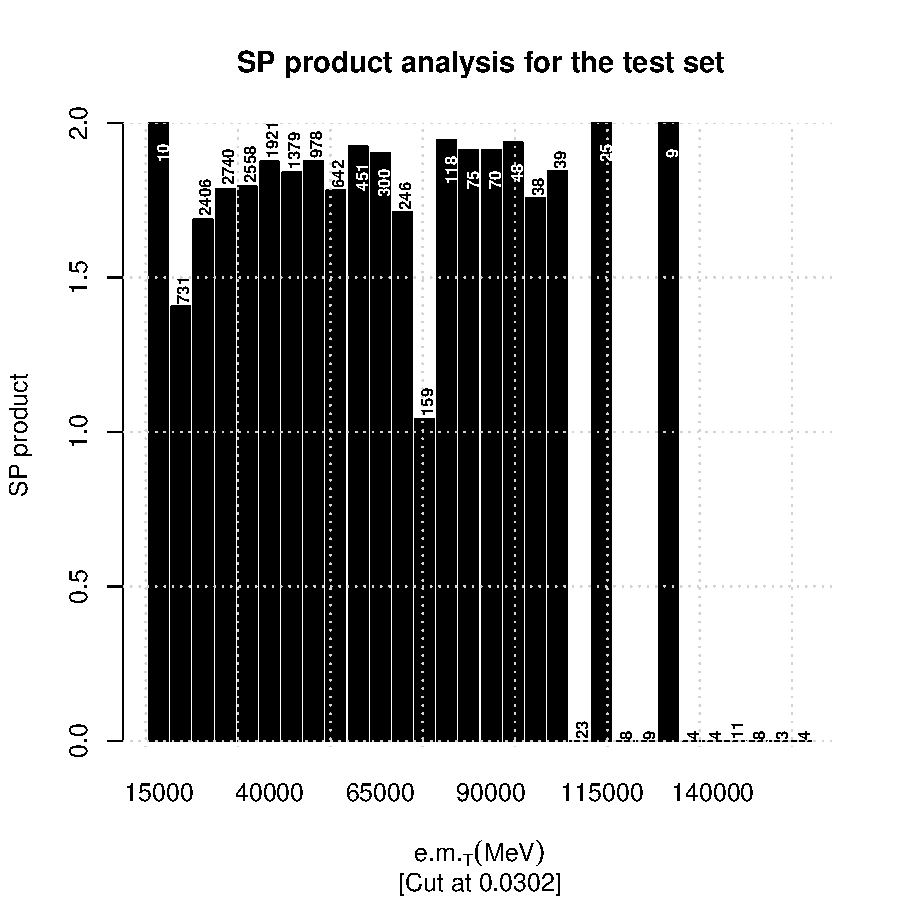
\includegraphics[scale=0.98]{lms/test-sp-emet}
\end{center}
\caption{Análise do produto SP por $\etem$.}
\label{fig:lms-test-sp-emet}
\end{figure}

\begin{figure}
\begin{center}
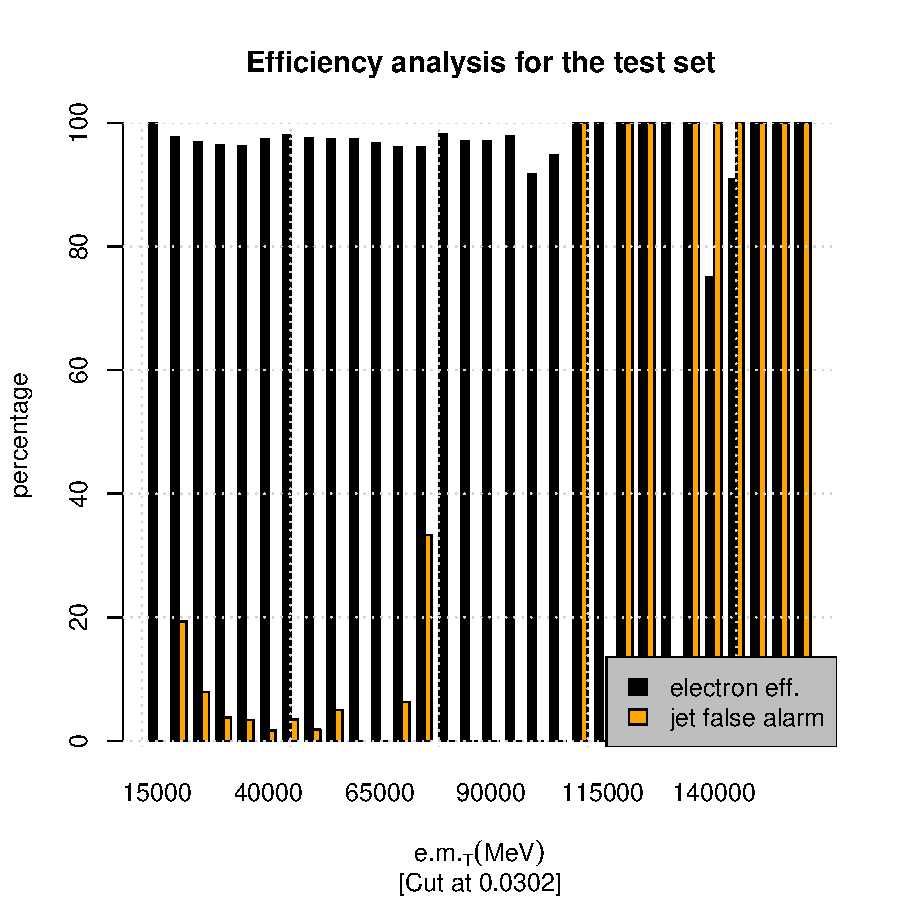
\includegraphics[scale=0.98]{lms/test-efficiency-emet}
\end{center}
\caption{Análise da eficiência de deteção de elétrons e falso alarme em jatos
para um detetor LMS, por $\etem$.}
\label{fig:lms-test-efficiency-emet}
\end{figure}

A Figura~\ref{fig:lms-vs-egamma} mostra um comparativo entre as duas técnicas
de deteção, por energia transversa na seção e.m.. Distingue-se que os dois
sistemas possuem respostas bastante próximas. Na primeira (mais à esquerda)
faixa de energia considerada, o EGammaHypo possui uma resposta melhor enquanto
que com o aumento da energia transversa o LMS apresenta-se mais eficiente, e
segue este padrão para quase todas as faixas consideradas, principalmente onde
há maior concentração de eventos de teste, como é possível determinar à partir
da Figura~\ref{fig:lms-test-sp-emet}.

\begin{figure}
\begin{center}
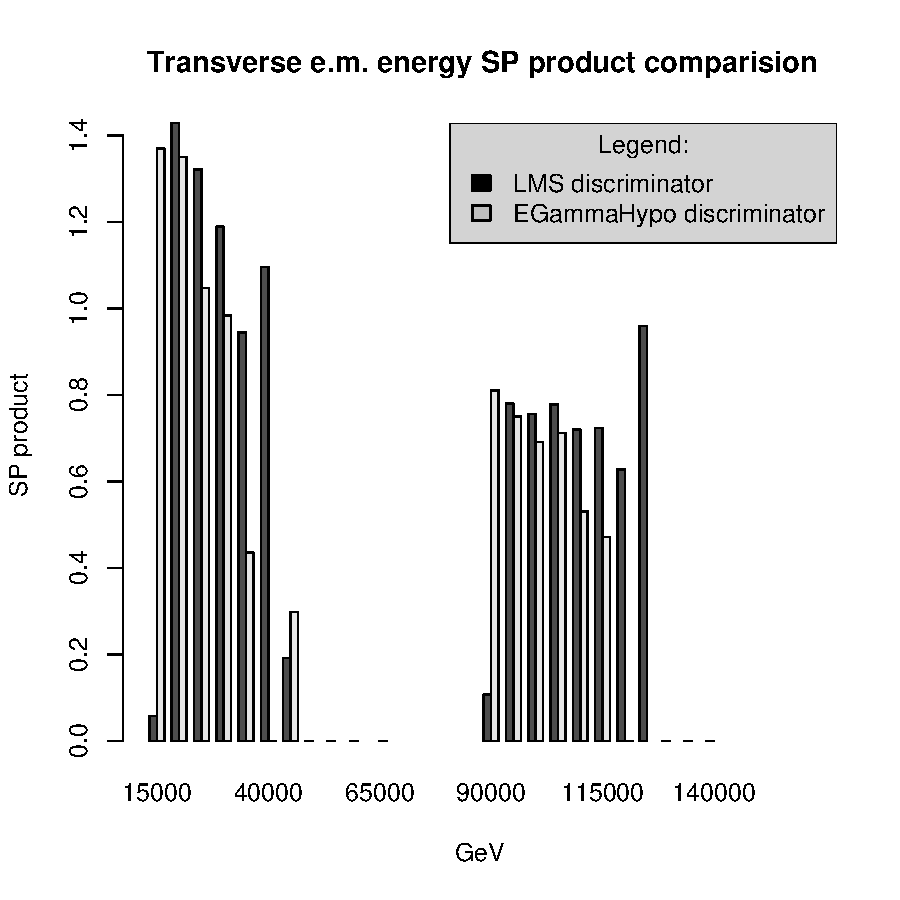
\includegraphics[scale=0.98]{lms/lms-vs-egamma}
\end{center}
\caption{Comparação do produto SP para um classificador baseado no LMS e o
EGammaHypo por energia transversa na seção e.m..}
\label{fig:lms-vs-egamma}
\end{figure}

\subsection{A relevância das características do T2Calo}

A técnica da análise de relevância \cite{relevance} tem por objetivo medir a
importância de cada uma das variáveis de entrada para um classificador. Nesta
técnica suprime-se a contribuição da variável à composição da saída
substituindo-se seu valor a cada evento por sua média, para todos os eventos
disponíveis na entrada do sistema de discriminação. Observando-se a variação
da saída, é possível estimar a contribuição daquela variável ao processo
discriminatório. A referência supracitada define a equação para a estimativa da
relevância da seguinte forma:

\begin{equation}
R_i = \frac{1}{N} \text{ } \overset{N}{\underset{j=1}{\sum}} \text{ }
[\text{saída}(\overrightarrow{x_j}) -
\text{saída}(\overrightarrow{x_j}\mid_{x_{j,i} = \overline{x}_i})]^2 
\label{eq:relevance-mse}
\end{equation}

Em outras palavras, é possível definir a relevância da variável $x_i$, $R_i$,
como o EMQ da saída de um discriminador comparado a mesma saída quando faz-se
a variável assumir o valor de sua média. Nessa equação, $N$ representa o
número total de eventos (padrões) disponíveis para o classificador, e $x_j$ um
evento particular. A Figura~\ref{fig:relevance-mse} mostra os valores de
relevância para cada uma das variáveis do classificador em análise. Esta
figura mostra mais uma vez que os conjuntos de teste e treino são
estatisticamente semelhantes, apresentando valores de relevância, para cada
uma de suas variáveis, bastante próximos. Ela também mostra que a variável
$\rcore$ é de extrema importância na determinação da saída do detetor. Quando
substituímo-la por sua média, o erro na saída aumenta de mais de 3 pontos
enquanto que para as demais variáveis, o impacto é nitidamente menor. Esta
figura também indica que a ordem de separação proposta pelo EGammaHypo está em
acordo com o processo de filtragem definido automaticamente pelo LMS,
levando-se em consideração a ordem onde os cortes são aplicados por aquele
algoritmo e a importância das variáveis nesse processo de classificação. A
importância destas variáveis ao sistema LMS poderia ser utilizada para
simplificá-lo. Por exemplo, seria possível ``podar'' a variável menos
relevante e re-treinar o sistema para obter um classificador mais rápido.

\begin{figure}
\begin{center}
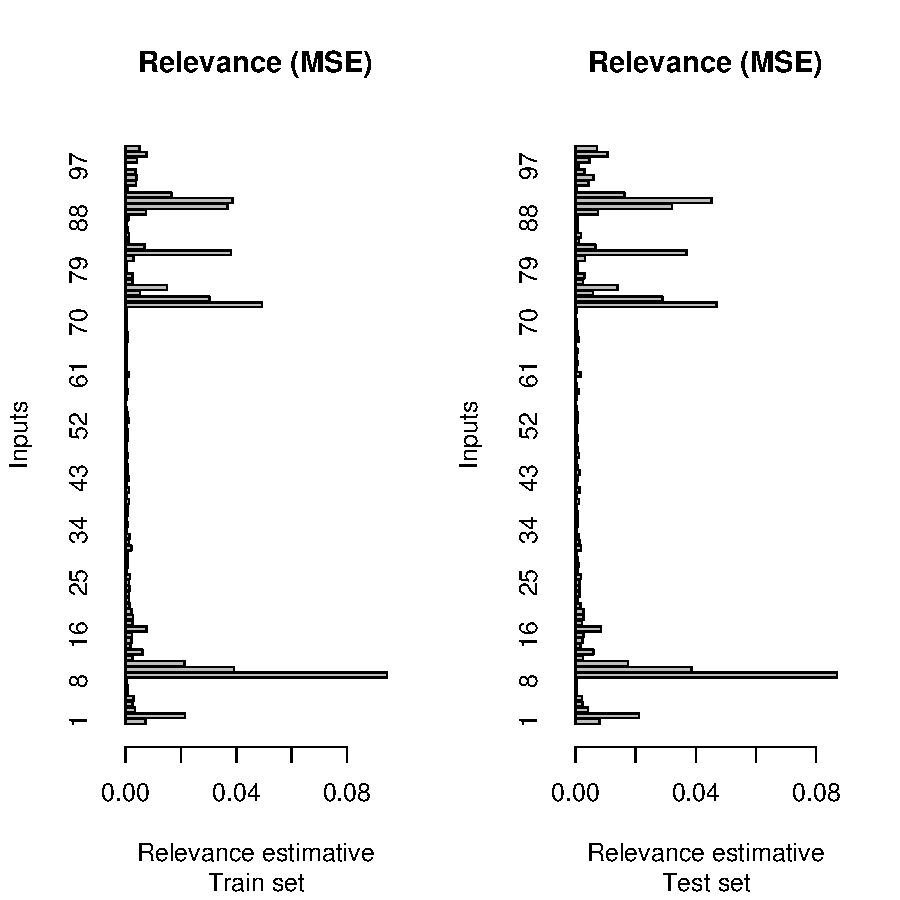
\includegraphics[scale=0.98]{lms/relevance-mse}
\end{center}
\caption{Os valores de relevância para os conjunto de treino (cinza claro) e
teste (em cinza escuro), para as 4 variáveis do T2Calo e considerando-se o
classificador LMS em estudo.}
\label{fig:relevance-mse}
\end{figure}

Por outro lado, como foi visto nas análises de evolução do EMQ
(Figura~\ref{fig:lms-mse-evo}) e do produto SP (Figura~\ref{fig:lms-sp-evo}),
a capacidade discriminatória da rede reage de forma correlacionada, mas
\textbf{não necessariamente} idêntica ao processo de mapeamento da entrada na
saída proposto pelo LMS. Observa-se que, apesar de notarmos uma contínua
migração ao mínimo EMQ durante cerca de 100 passos de treinamento, após cerca
de apenas 20 passos, a capacidade discriminatória do sistema já atinge seu
máximo e ali permanece até o final do treinamento. Este comportamento indica
que exista uma diferença fundamental entre estes dois parâmetros. Portanto,
seria de pouca prudência considerarmos apenas o valor de relevância proposto
para a avaliação da importância de cada variável \underline{ao processo
discriminatório}. Desta forma, propõe-se uma variação do cálculo da relevância,
mas agora baseando-se no impacto da substituição do valor da variável pela sua
média à capacidade discriminatória da rede. Naturalmente nos utilizaremos do
produto SP para o cálculo da relevância de discriminação do LMS, da seguinte
forma:

\begin{equation}
R_{d_i} = \max(\text{SP}) - \max(\text{SP}(\overrightarrow{x_j}\mid_{x_{j,i} = \overline{x}_i}))
\label{eq:relevance-sp}
\end{equation}

Neste caso define-se a \textit{Relevância de Discriminação da variável $i$},
ou $R_{d_i}$, de uma variável $i$ como a diferença no produto SP máximo
causado pela substituição desta variável pela sua média. De fato, espera-se
que a maior parte dos valores de relevância sejam positivos, indicando uma
degradação do desempenho do classificador seguindo a neutralização de uma
variável. Embora improvável no caso corrente, seria, num geral, possível
encontramos valores de relevância negativos, o que indicaria que uma variável
está, na verdade, atrapalhando o processo de classificação ao invés de
melhorá-lo. A Figura~\ref{fig:relevance-sp} mostra os valores de $R_d$ para o
classificador LMS em estudo. Como é possível ver nesta figura, o quadro é
marginalmente diferente daquele mostrado pela
Figura~\ref{fig:relevance-mse}. A variável mais importante para o processo
discriminatório é ainda $\rcore$, seguindo-se de $\eratio$ e $\ethad$. A
variável $\etem$ é a menos relevante para o processo de classificação de
elétrons e jatos, o que já era esperado observando-se as tendências
anteriores. Observa-se também que, embora haja concordância nos resultados
para dentro de um mesmo subconjunto de dados (treino \textit{versus} teste),
os resultados apresentam-se ligeiramente mais discrepantes que para outras
figuras de mérito, principalmente para a variável $\eratio$. Como é possível
definir à partir deste gráfico, seria preferencial uma poda da variável
$\etem$ que da variável $\ethad$, como sugeriria a
Figura~\ref{fig:relevance-mse}. No mais, as duas figuras são bastante
compatíveis e indicam uma tendência importante: a minimização do EMQ também
maximizará o produto SP. Esta figura também indicaria que a ordem na qual o
EGammaHypo considera as variáveis de corte (i.e. $\rcore \rightarrow
\eratio \rightarrow \etem \rightarrow \ethad$) seja não-ótima, mesmo que
marginalmente. Observa-se que seria mais interessante que o corte em $\etem$
fosse realizado por último ao invés do corte em $\ethad$.

\begin{figure}
\begin{center}
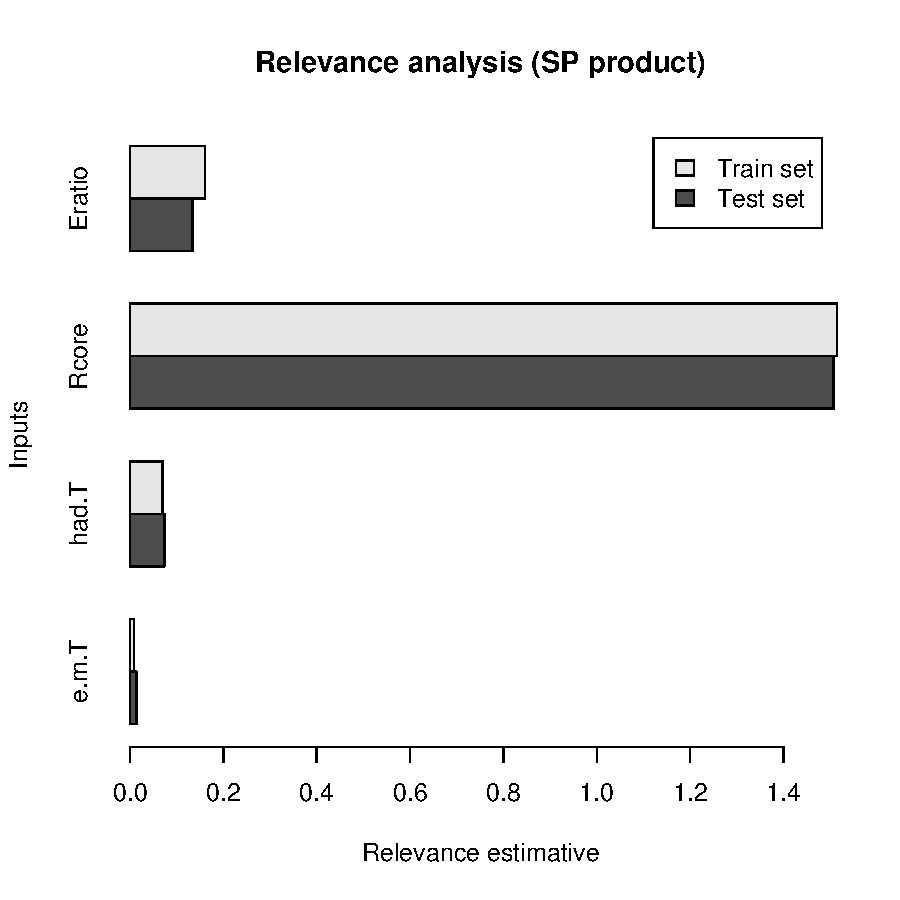
\includegraphics[scale=0.98]{lms/relevance-sp}
\end{center}
\caption{Os valores de Relevância de Discriminação para os conjunto de treino
(cinza claro) e teste (em cinza escuro), para as 4 variáveis do T2Calo e
considerando-se o classificador LMS em estudo.}
\label{fig:relevance-sp}
\end{figure}

\section{Métodos Neurais de Discriminação}
\label{sec:neural}

Redes neurais artificiais (RNA) vem sendo atualmente utilizadas com sucesso em
problemas de otimização, controle e reconhecimento de padrões
\cite{haykin}. RNA's são modelos matemáticos inspirados no conhecimento
limitado que temos do cérebro animal. Neste contexto, entende-se que uma rede
neural pode aprender através do contato com os elementos de interesse de um
determinado espaço de entrada e que este conhecimento é armazenado através das
conexões sinápticas que conectam os elementos processadores (neurônios) da
rede. Dentre as características de uma RNA podemos destacar:

\begin{description}
\item[Robustez] Em ambientes extremamente \emph{agressivos} (sujeitos a falhas
e a radioatividade), como é o caso da operação do ATLAS, RNA's podem manter um
excelente desempenho, mesmo quando parte dos dados (canais de aquisição) de
entrada são perdidos;

\item[Generalização] RNA's podem extrair a informação relevante escondida sob
uma grande quantidade de ruído;

\item[Deteção de novos fenômenos] RNA's podem detetar a ocorrência de novos
objetos de forma bastante eficaz. Isto é \underline{extremamente} importante
em ambientes que podem revelar resultados inesperados (nova física);

\item[Simples implementação] RNA's podem ser facilmente descritas em
linguagens de programação convencionais, atingindo desempenhos satisfatórios
para um grande conjunto de aplicações em tempo real.
\end{description}

A utilização de RNA's em experimentos em Física de Altas Energias também vem
se popularizando ao longo das últimas década, principalmente na área de
calorimetria, tanto especificamente em sistemas de filtragem \cite{badgett92,
koehne96} quanto para análise pós-reconstrução \cite{altherr90}. Isto se deve
principalmente ao fato que RNA's consigam definir uma superfície de separação
não-linear no espaço de dados sendo considerado, normalmente atingindo
resultados bastante acurados na determinação do \eng{background} e ainda
retendo um desempenho satisfatório quando comparadas às técnicas de deteção
por cortes como as discutidas anteriormente (veja a
Seção~\ref{sec:def-eghypo}).

\subsection{Introdução ao processamento neural}

A Figura~\ref{fig:neuron} contém uma modelagem de um neurônio
genérico. Analogamente ao sistema LMS descrito na Seção~\ref{sec:lms}, os
elementos processadores de uma rede neural, chamados neurônios ou percéptrons,
são ativados por um conjunto de entradas $\overrightarrow{x}$, somadas de
acordo com um sistema linear de pondeção $\overrightarrow{w}$. O diferencial
entre o sistema linear proposto anteriormente e um neurônio está na função de
ativação que conduz o campo induzido $v_p =
\overrightarrow{x}*\overrightarrow{w}_{p}^{T}$ à saída. Enquanto que
no caso do LMS utiliza-se a função identidade, i.e., $y_p = v_p$, no caso de
percéptrons, faz-se uso de uma função não-linear, como por exemplo a função
tangente hiperbólica:

\begin{figure}
\begin{center}
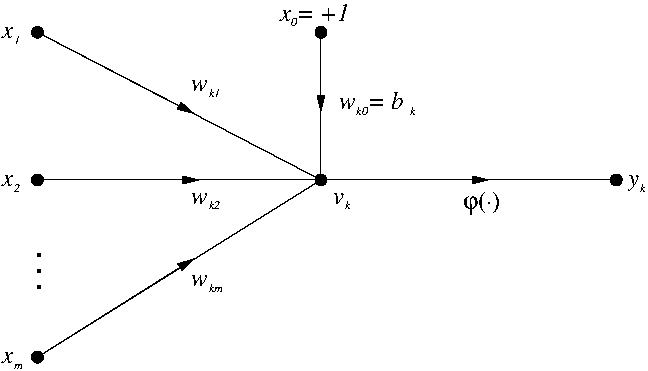
\includegraphics{neuron}
\end{center}
\caption{Grafo de fluxo de sinal de um neurônio artificial.}
\label{fig:neuron}
\end{figure}

\begin{equation}
tanh(v) = \frac{e^v - e^{-v}}{e^v + e^{-v}} = \frac{e^{2v} - 1}{e^{2v} + 1}
\label{eq:tanh}
\end{equation}

Ou a função logística (simplificada):

\begin{equation}
P(v) = \frac{1}{1 + e^{-v}}
\label{eq:logf}
\end{equation}

A razão da escolha de uma função não-linear para a ativação de um campo
induzido pode ser qualificado à partir da seguinte constatação: se sistema a
que se deseja classificar aprensenta um comportamento gaussiano, para ambas as
classes, i.e., os momentos de ordem superior a $2$ para ambas as classes são
todos iguais a zero, o classificador ótimo (bayesiano) resume-se um sistema
linear \cite{haykin}. Naturalmente nota-se que seja sempre possível
\textit{aproximar} ou modelar um sistema não-gaussiano em um desta espécie,
tendo por conseqüência os erros relativos a esta aproximação. De fato, foi o
que foi realizado na Seção~\ref{sec:lms-ej}, quando escolhemos um
classificador linear para separar as quatro variáveis definidas pelo T2Calo.

Se o sistema que se deseja resolver apresenta um comportamento não-gaussiano,
o classificador ótimo não pode ser representando por um classificador
linear. Neste caso, utiliza-se uma função de ativação não-linear para que se
aproxime, de alguma forma, o comportamento não-linear do sistema de interesse.
Assim sendo, as funções nas Equações~\ref{eq:tanh} e \ref{eq:logf} são
normalmente utilizadas por apresentarem amplitude limitada e possuírem
derivada trivialmente calculável. A razão de procurar-se funções com derivadas
simples (e suaves) ficará mais clara adiante, quando se definir o algoritmo de
treinamento. A amplitude limitada pode rapidamente ser verificada como uma
característica de interesse observando-se que o treinamento de um sistema que
trabalha por aprendizado seja muitas vezes executado com a retro-alimentação
de erros. Neste caso, para evitar oscilações e pontos de ressonância, um
sistema cuja a saída seja limitada apresenta natural vantagem se comparado a
outro análogo.

Este estudo está focado na utilização de RNA's utilizando percéptrons em
múltiplas camadas (do inglês \eng{Multi-layer perceptrons} ou MLP),
completamente conectadas, sem realimentação e com treinamento baseado na
retropropagação de erros. Introduziremos o processo de treinamento destes
sistemas à seguir.

\subsection{Treinamento por retro-propagação de erros}

Para sistemas com apenas uma camada neural, observa-se que ao buscar-se o
ponto de mínimo da superfície de erro (quadrático), naturalmente otimiza-se o
conjunto de pesos de tal forma que o sistema tente mapear de forma ótima a
entrada nos alvos de saída. A única restrição do método é que a função de
ativação do campo induzido do neurônio $\varphi(\cdot)$ seja diferenciável.
\cite{rosenblatt}. O problema do treinamento de uma rede MLP é um pouco mais
complexo. Um grafo de fluxo de uma rede MLP completamente conectada pode ser
visto na Figura~\ref{fig:simple-mlp}. Neste caso considera-se que a rede
possui apenas uma camada escondida e apenas um neurônio de saída pois se
identifica intimamente com os casos de uso que abordaremos. Ainda sim, seria
possível considerar casos com um número maior de neurônios de saída ou com
mais camadas escondidas generalizando os casos exemplificados aqui.

\begin{figure}
\begin{center}
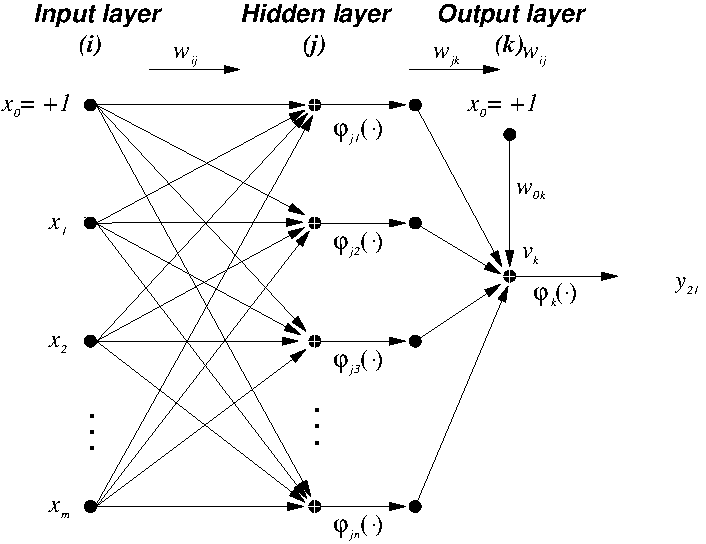
\includegraphics{simple-mlp}
\end{center}
\caption{Modelagem de uma rede MLP, totalmente conectada e sem
retro-propagação de sinal.}
\label{fig:simple-mlp}
\end{figure}

Para o sistema em questão, o mecanismo de treinamento para o neurônio de saída
é idêntico ao treinamento de um percéptron simples, e pode ser facilmente
definido da seguinte forma:

\begin{align}
\text{Se define-se o erro como } \mathcal{E}(n) &= \frac{1}{2}e_{k}^{2}(n)
\label{eq:error-def} \\
\text{e considerando-se que } \frac{\partial\mathcal{E}(n)}{\partial
w_{jk}(n)} &= \frac{\partial\mathcal{E}(n)}{\partial e_k(n)} \frac{\partial
e_k(n)}{\partial y_k(n)} \frac{\partial y_k(n)}{\partial v_k(n)}
\frac{\partial v_k(n)}{\partial w_{jk}(n)} \label{eq:partials} \\
\text{ou seja, } \frac{\partial\mathcal{E}(n)}{\partial
w_{jk}(n)} &= e_k(n)(-1)\varphi_{k}'(v_{k}(n))y_{k}(n)
\label{eq:partials-solution} \\
\text{e, resumindo, } \Delta w_{jk}(n) &=
-\eta\frac{\partial\mathcal{E}(n)}{\partial w_{jk}(n)} = \eta
e_{k}(n)\varphi_{k}'(v_{k}(n))y_{k}(n)
\end{align}

Normalmente nota-se:

\begin{align}
\text{Gradiente local: } \delta_k(n) &= - e_k(n)\varphi_{k}'(v_k(n)) \\
\text{e desta forma } \Delta w_{jk}(n) &= \eta\delta_k(n)y_{k}(n)
\label{eq:neural-train}
\end{align}

Este sistema de equações segue o princípio definido anteriormente para o LMS,
mas sem assumir nada sobre a função de ativação $\varphi(\cdot)$. Nota-se que
para uma função de ativação onde $y_k(n) = v_k(n)$, recai-se no algoritmo de
treinamento do LMS: $\Delta w_{jk}(n) = \eta e_{j}(n)y_{j}(n)$. Desta forma, é
possível considerar o LMS como um caso especial de uma rede neural com apenas
uma camada cuja a função de ativação é a função identidade. Nestas equações,
$n$ representa a época ou batelada de treinamento.

O segundo caso de interesse acontece quando o neurônio $j$ está localizado em
uma camada oculta da rede. Neste caso, não existe uma resposta desejada (alvo)
específica para aquele neurônio. Desta forma, tentar-se-á definir o sinal de
erro de um neurônio escondido recursivamente, através da retro-propagação do
erro na saída final da rede em direção ao neurônio desejado. Iniciamos,
intuitivamente, com a definição do gradiente local do neurônio escondido $j$:

\begin{equation}
\delta_j(n) = -\frac{\partial\mathcal{E}(n)}{\partial
v_j(n)} = -\frac{\partial\mathcal{E}(n)}{\partial
y_j(n)}\frac{\partial y_j(n)}{\partial v_j(n)} =
-\frac{\partial\mathcal{E}(n)}{\partial y_j(n)}\varphi_{j}'(v_j(n))
\end{equation}

Tendo em conta, que para o caso específico em análise:

\begin{align}
\mathcal{E}(n) &= \frac{1}{2}e_{k}^{2}(n) \\
\text{conclui-se que } \frac{\partial\mathcal{E}(n)}{\partial y_j(n)} &=
e_{k}\frac{\partial e_k(n)}{\partial y_j(n)} = e_{k}\frac{\partial
e_k(n)}{\partial v_k(n)}\frac{\partial v_k(n)}{\partial y_j(n)}
\end{align}

A primeira derivada parcial, $\partial e_k(n)/\partial v_k(n)$, já foi
calculada para o caso do neurônio de saída, na passagem da
Equação~\ref{eq:partials} para a
Equação~\ref{eq:partials-solution}. Utiliza-se a mesma analogia aqui. Para o
cálculo da segunda derivada parcial, pela Figura~\ref{fig:simple-mlp}
deduz-se que:

\begin{align}
v_k(n) &= \sum_{j} w_{jk}(n)y_j(n) \\
\text{e, portanto: } \frac{\partial v_k(n)}{\partial y_j(n)} &= w_{jk}(n)
\end{align}

Assim sendo, o gradiente local do neurônio escondido $j$ assim se define:

\begin{equation}
\delta_j(n) = \varphi_{j}'(v_j(n))\delta_k(n)w_{jk}(n)
\label{eq:local-gradient-hidden}
\end{equation}

Substituindo $\delta_j(n)$ na Equação~\ref{eq:neural-train}, chega-se a
fórmula de treinamento do neurônio escondido. No caso onde há muitas saídas na
rede, a Equação~\ref{eq:local-gradient-hidden} é trivialmente redefinida da
seguinte forma: 

\begin{equation}
\delta_j(n) = \varphi_{j}'(v_j(n))\sum_{k}\delta_k(n)w_{jk}(n)
\label{eq:local-gradient-hidden-multi}
\end{equation}

No caso em que existem múltiplas camadas escondidas, propaga-se recursivamente
o erro em direção à camada de entrada, aplicando-se a
Equação~\ref{eq:local-gradient-hidden-multi}. 

\subsubsection{Funções de ativação} 

A função de ativação $\varphi(\cdot)$ deve ser diferenciável em toda a
extensão do domínio de interesse. No entanto, para simplificar o cálculo
computacional dos gradientes locais, é habitual a escolha de funções que
possuam um cálculo trival de suas derivadas. Como exemplo, foram citadas as
funções tangente hiperbólica (Equação~\ref{eq:tanh}) e a função logística
simplificada (Equação~\ref{eq:logf}). No caso da função logística:

\begin{align}
\varphi(z) &= \frac{1}{1 + e^{-z}} \\
\text{Daí } \varphi'(z) &= \frac{e^{-z}}{[1+e^{-z}]^2}
\end{align}

Levando-se em consideração que para um neurônio genérico $y =
\varphi(v)$. Então:

\begin{equation}
\varphi'(v) = \frac{e^{-v}}{[1+e^{-v}]^2} = \frac{1+e^{-v}}{[1+e^{-v}]^2} -
\frac{1}{[1+e^{-v}]^2} = \varphi(v)[1 - \varphi(v)] = y(1-y)
\end{equation}

No caso da tangente hiperbólica, equivalentemente:

\begin{align}
\varphi(z) &= \tanh(z) \\
\varphi'(z) &= \text(sech)^2(z) = 1 - \tanh^2(z) \\
\varphi'(v(n)) &= 1 - \varphi^2(z) = 1-y^2(n)
\end{align}

Estas duas funções de ativação permitem um cálculo absolutamente trivial do
gradiente local e por esta razão são computacionalmente bastante
eficientes. No decorrer deste estudo utilizaremos a função tangente
hiperbólica com função de ativação dos percéptrons das redes estudadas.

\subsubsection{Convergência}

O algoritmo de retropropagação usa uma estimativa instantânea para o gradiente
da superfície de erro no espaço dos pesos. Por esta razão, este sistema possui
uma inerente natureza estocástica e tende a oscilar ao redor da direção de
convergência ótima, ao mínimo da função de erro. Isso acontece pois é difícil
antever se inclinações demasiado bruscas ou suaves em uma das direções da
superfície de erro não influenciarão excessivamente o deslocamento do
sistema. Muitas vezes, a utilização de um amortecimento (ou \emph{momento})
durante o treinamento pode melhorar a resposta do sistema. Utilizaremos esta
técnica para suavizar a migração das redes em direção ao mínimo da superfície
de erro. Outra técnica que será empregada é a normalização dos dados de
entrada da rede, de forma que se evite que a diferença de magnitude e
variabilidade das componentes de entrada polarizem o treinamento neural.

Outro problema recorrente são mínimos locais, que podem fazer com que o
sistema fique ``preso'' em uma região que não represente o mínimo global da
superfície de erro. Esta característica não é somente mais uma conseqüência da
utilização da estimativa instantânea para definir a direção de movimentação
dos pesos, mas muitas vezes ocorre por dispor-se de uma quantidade limitada de
eventos que representem o fenômeno que se deseja mapear.

Para que se assegure de que o sistema converge sempre a um patamar equivalente
de mínimo, realizar-se-á um número de experimentos com os mesmos parâmetros de
treinamento e teste para todos os casos de estudo. Em cada teste inicializa-se
os pesos sinápticos à partir de um ponto diferente da superfície de
erro. Desta forma, será possível detetar e avaliar se o problema em estudo
estará sujeito a mínimos locais.

\subsection{\textit{NeuralRinger}: Projeto e implementação}
\label{sec:framework}

O \textit{NeuralRinger} é um pacote totalmente desenvolvido usando o paradigma
da orientação à objetos, implementado em C++ \cite{stroustrup} e especialmente
concebido para executar a operação de filtragem de partículas dentro do
LVL2. Outras soluções para treinamento e execução de redes neurais, tais como
o pacote SNNS \cite{snns} foram investigadas antes do desenvolvimento deste
sistema. Entrentanto, os pacotes em questão são normalmente utilizados para
uma grande variedade de sistemas neurais. Esta flexibilização muito
freqüentemente ocorre em detrimento do desempenho em casos
específicos. Ademais, ao usar um sistema tão genérico, se estaría inserindo
uma grande quantidade de código dentro do sistema de filtragem que seria, em
sua maior parte, desprezada.

As escolhas do paradigma de programação e da linguaguem de implementação C++
ocorreram em função do ambiente-alvo para este sistema. Como colocado na
Seção~\ref{sec:hlt}, o LVL2 de filtragem rodará utilizando como base as
bibliotecas do Projeto Athena. O Athena é o \eng{framework} padrão para a
análise da Física dos eventos no ATLAS, tanto no Sistema de Filtragem, como na
Reconstrução pós-filtragem nos diversos \eng{clusters} de análise
\eng{offline} e análise dos resultados. Desta forma, a integrabilidade ao Athena
constitui-se de um passo essencial para a utilização da técnica no LVL2.

Este pacote foi desenvolvido tendo por base as seguintes prerrogativas, em
ordem:

\begin{enumerate}
\item Otimização do passo de execução de redes: É importante que o sistema
tenha o menor tempo possível para a execuação do processamento neural, de tal
forma que seja viável a execução no sistema de filtragem. Preferencialmente,
deseja-se que 1 passo de execução da rede não dure mais que 1~ms, já que o
tempo total de processamento no LVL2 deva ser, em média 10~ms, contando com o
acesso aos dados;
\item Interoperabilidade: O treinamento do sistema deve ser executado
\eng{offline}, dada a disponibilidade dos dados. Portanto, é necessário que o
sistema opere tanto dentro do \eng{framework} Athena quanto em modo
desconectado;
\item Multi-tarefas: Respeitando o projeto do LVL2, o \eng{NeuralRinger} não
deve ter construções que impossibilitem ou dificultem a sua utilização
concorrente em múltiplas tarefas;
\item Configurabilidade: O \eng{NeuralRinger} deve ser, dentro de determinadas
medidas, configurável e flexível com relação ao treinamento dos pesos
sinápticos e a configuração da rede que será usada na deteção dos alvos. O
método de treinamento a ser utilizado será a retro-propagação de erros, tendo
por base redes totalmente conectadas e sem re-alimentação.
\end{enumerate}

\subsubsection{Projeto}

O projeto do \eng{NeuralRinger} está dividido em quatro pacotes que executam
funções bem-definidas para o interfaceamento, configuração e execução de redes
neurais. A Figura~\ref{fig:nr-packages} contém um diagrama UML (do inglês,
\eng{Unified Modelling Language}, \cite{booch}) nomeando e
mostrando a relação de dependência entre estes pacotes.

\begin{figure}
\begin{center}
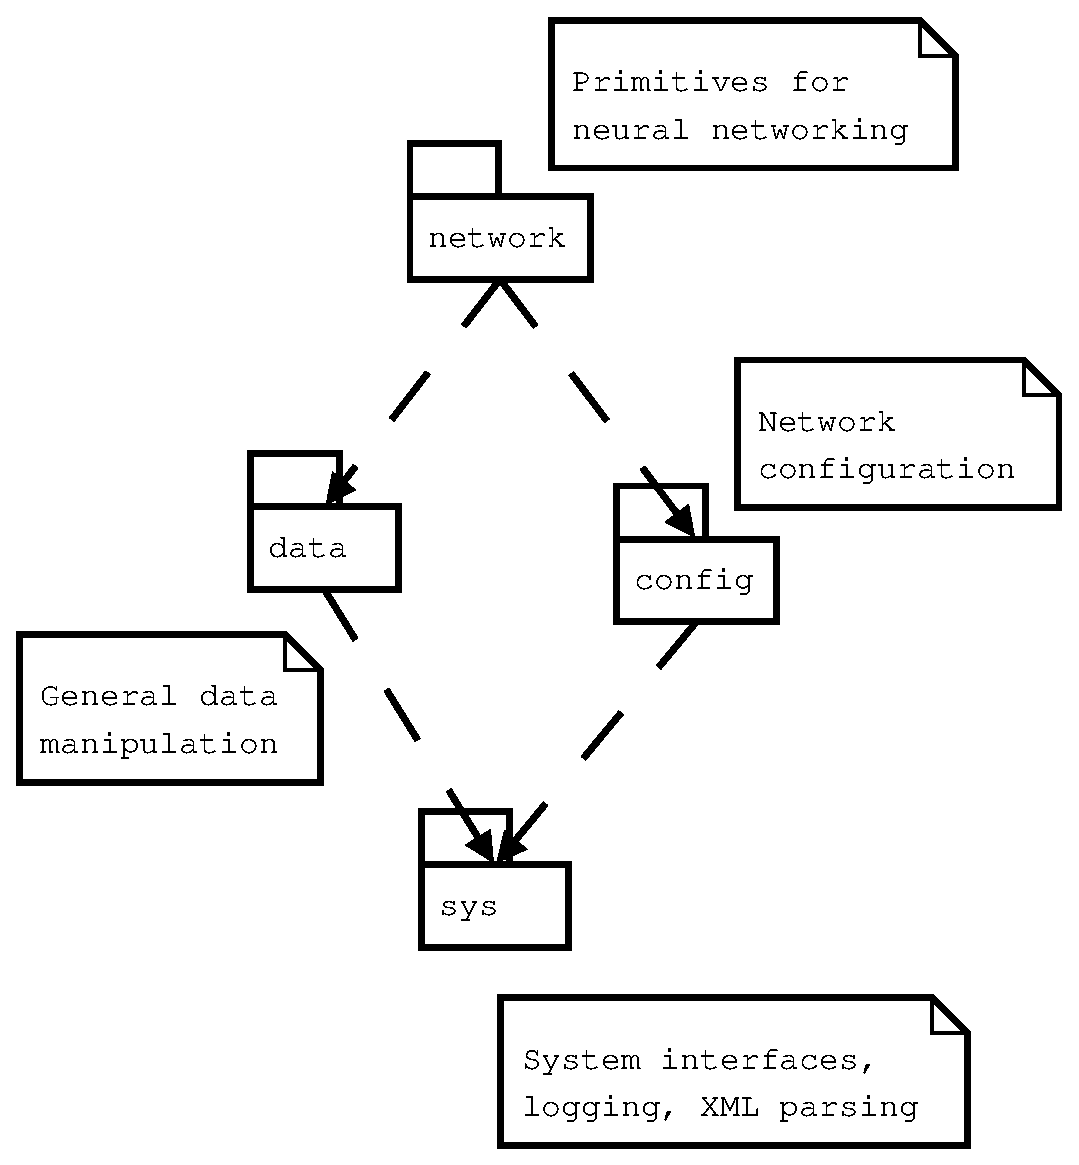
\includegraphics[scale=0.4]{nr-packages}
\end{center}
\caption{Diagrama de blocos mostrando a relação entre os pacotes do
\eng{NeuralRinger}.}
\label{fig:nr-packages}
\end{figure}

\paragraph{\texttt{SYS}:} O pacote \texttt{sys} está abaixo na cadeia de
dependências e não depende em nenhum outro pacote do projeto. Este pacote
inclui ferramentas para a manipulação de formatos XML e um sistema básico para
o relatório de erros. A escolha da linguagem XML como formato de troca de
dados e valores de configuração sucede-se da grande quantidade de
interpretadores (\eng{parsers}) disponíveis livremente na \eng{internet}, já
que é um padrão bastante difundido. O suporte a XML disponível atualmente
inclui, mas não se limita a verificações de sintaxe automatizadas (via
\eng{XML schemas}) e transformações para que se adicione informação ao seja
possível a visualização de forma adequada do conteúdo de uma base de dados
XML.

A Figura~\ref{fig:sys-uml} traz uma visão geral dos componentes e seu
relacionamento dentro deste pacote. Na parte central do diagrama encontramos o
tipo \texttt{Reporter} que define uma interface para o relatório de
erros. Objetos deste tipo contém uma implementação específica do sistema de
relatório de erros. Inicialmente, somente a implementação baseada em
arquivos-padrão tais como \texttt{std::cout} e \texttt{std::cerr}
\cite{web:gcc-stl} foi desenvolvida. À direita observa-se a modelagem para o
sistema de interpretadores XML. Uma interface (abstrata) é utilizada como base
para implementações específicas baseadas em interpretadores habitualmente
encontrados nos sistemas operacionais correntes. Especificamente,
implementações para o sistema Xerces C++ \cite{xerces-c}, do grupo Apache e
libxml2 \cite{libxml2}, do grupo Gnome estão presentes na implementação
atual. O interpretador XML utiliza-se do sistema de relatório de erros para
relatar problemas na leitura ou escrita de arquivos de forma unificada. Uma
caixa de ferramentas, baseada no tipo abstrato \texttt{XMLProcessor} provê um
conjunto primitivas para facilitar a escrita e leitura de parâmetros e trechos
de texto. No evento de erros fatais, uma exceção baseada no tipo
\texttt{Exception} será lançada pela parte afetada do código.

\begin{figure}
\begin{center}
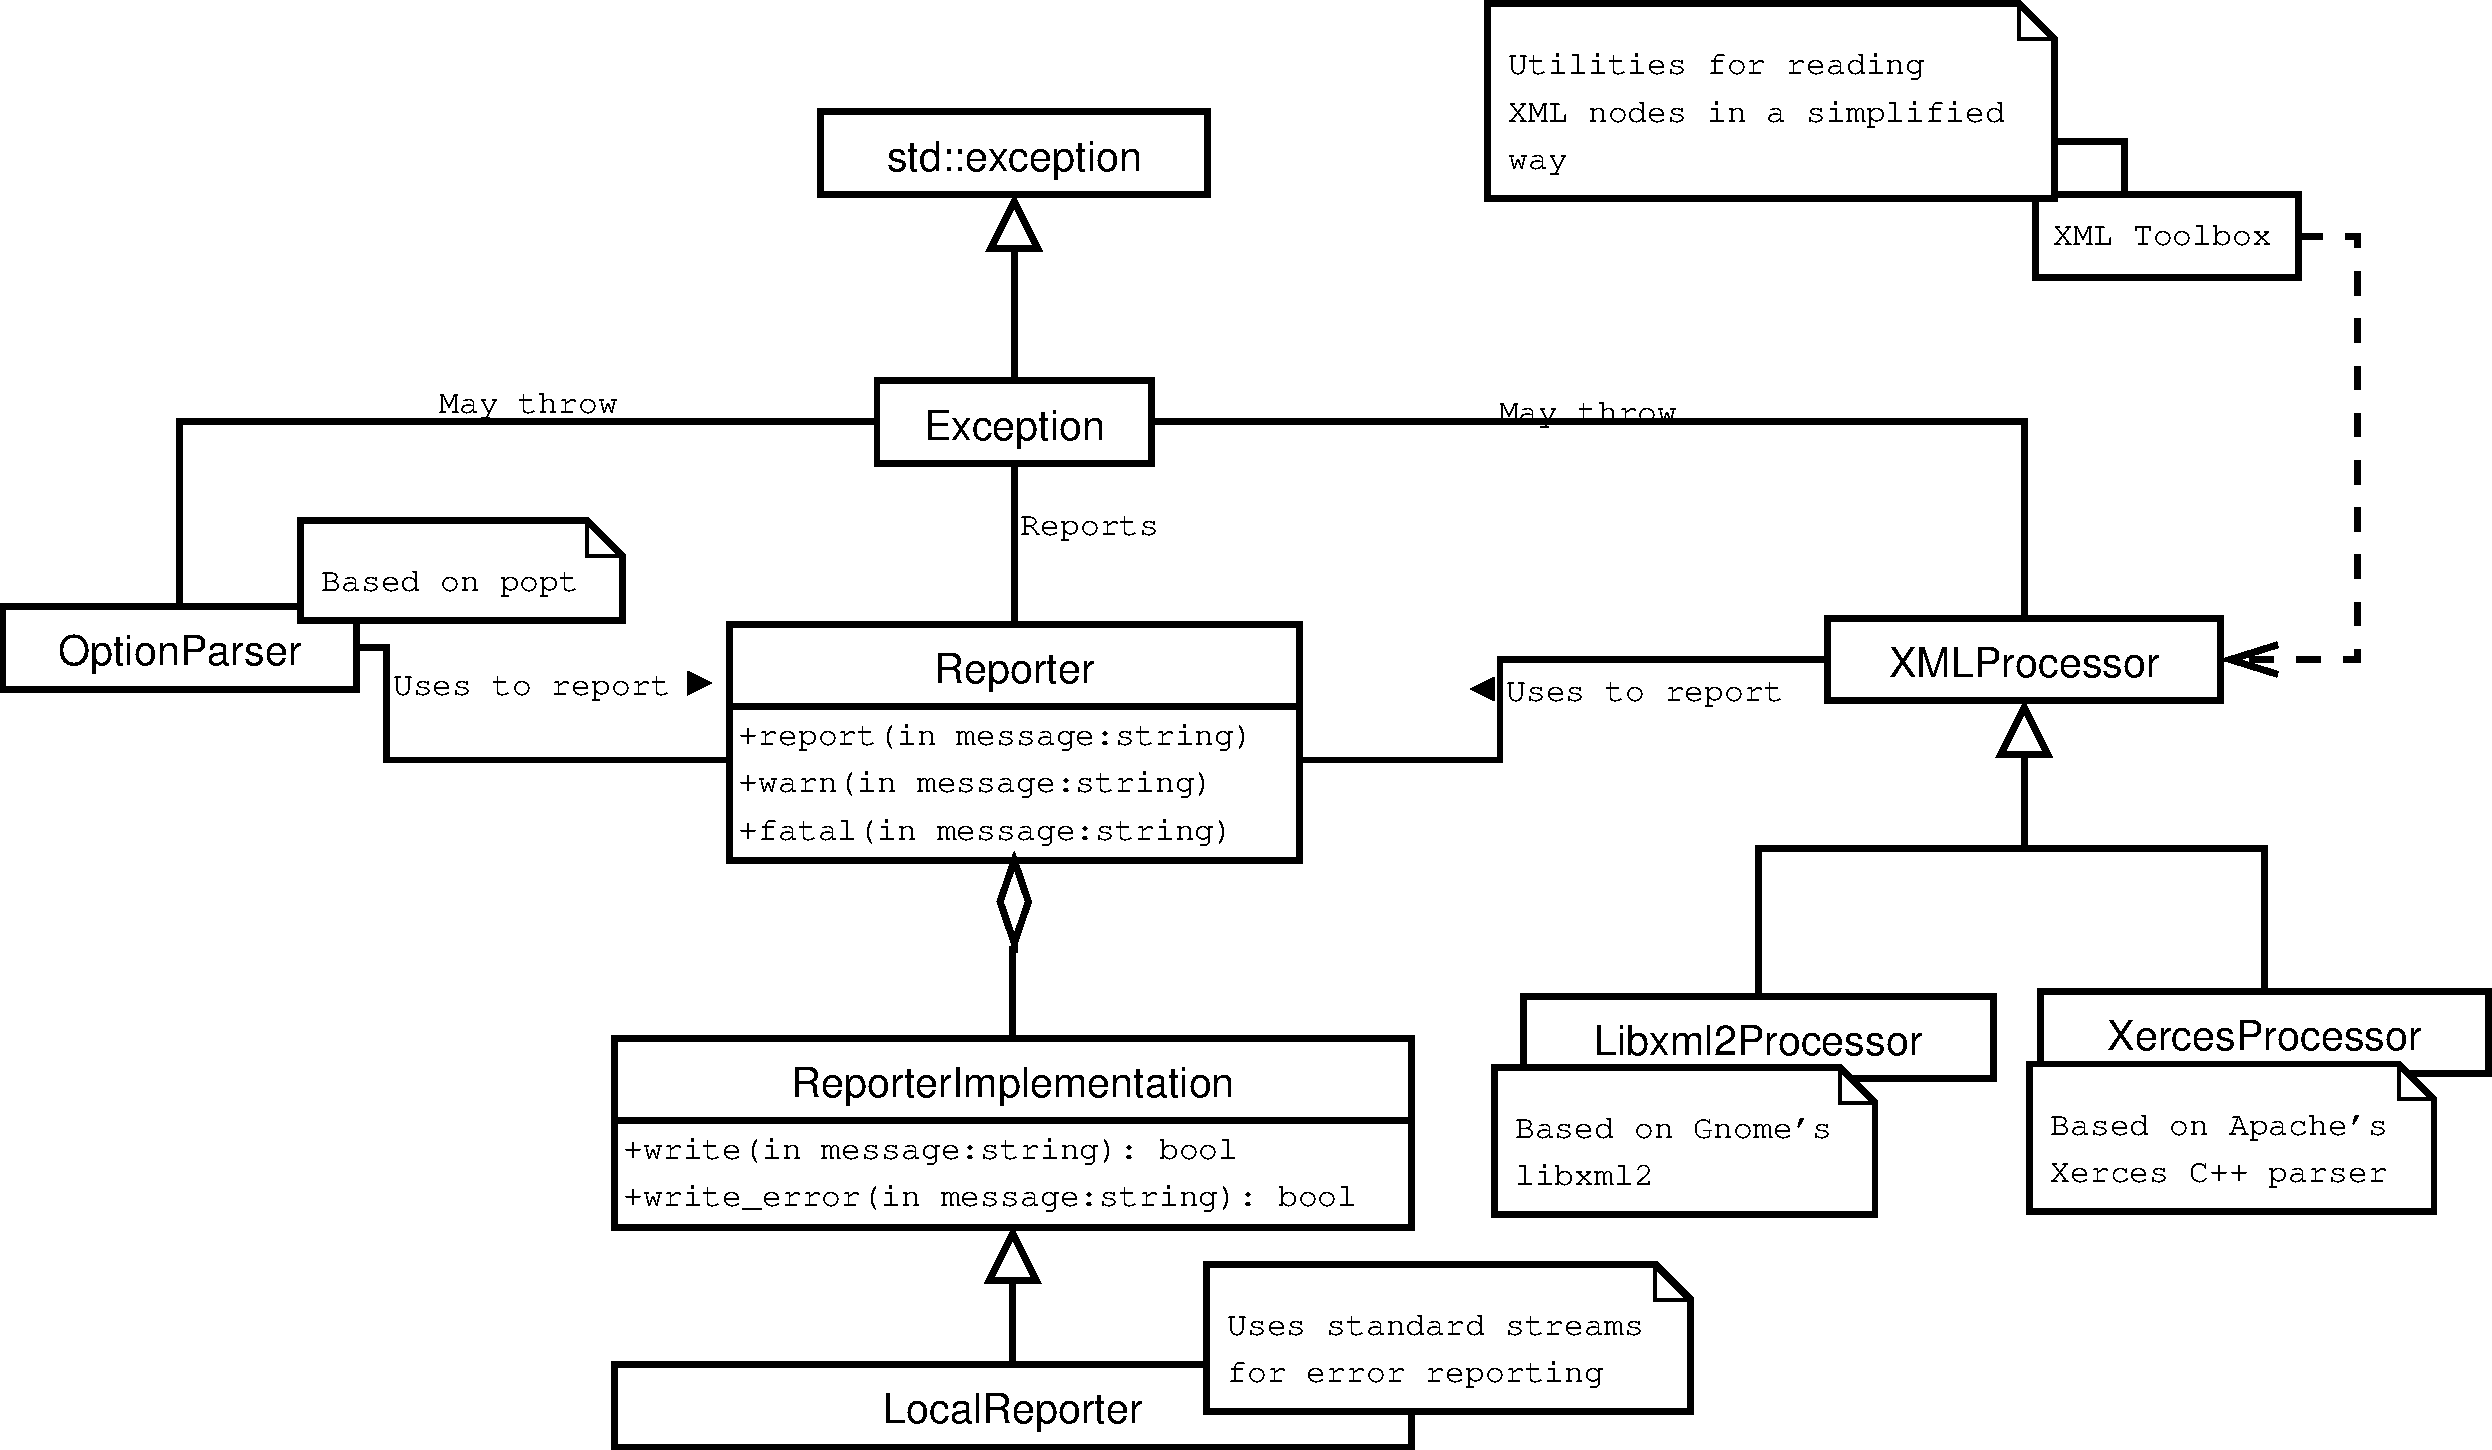
\includegraphics[scale=0.3]{sys-uml}
\end{center}
\caption{Diagrama UML mostrando as relações dos componentes do pacote
\texttt{sys}.}
\label{fig:sys-uml}
\end{figure}

O pacote \texttt{sys} também fornece um sistema para a interpretação de opções
de linha de comando, baseado no interpretador \texttt{popt}. Este tipo imbute
um sistema de atribuição automática e checagem de valores, conectando as
opções na linha de comando diretamente com o contexto onde as opções serão
utilizadas dentro do programa. Seguindo a filosofia dos interpretadores XML,
este tipo também faz uso do sistema central de relatório de erros para
informar problemas ao usuário e poderá, no caso de problemas sérios, também
lançar exceções de operação.

\paragraph{\texttt{DATA}:} O pacote \texttt{data} contém as primitivas para a
manipulação dos dados, prévia e posteriormente ao processamento neural. Ele
utiliza as primitivas definidas no pacote \texttt{sys} para executar a
reportagem de erros, lançamento de exceções ou a leitura de arquivos XML. A
Figura~\ref{fig:data-xml} contém um diagrama mostrando a relação das classes
dentro do pacote \texttt{data}.

\section{Mapeamento topológico}

Fazer uma descrição detalhada do sistema que mapeia em anéis, a informação da
RoI. Aplicação de uma rede neural como discriminador (hipótese).

\subsection{Análise física}

Esta seção vai falar do desempenho "físico" do neuralringer. Quão melhor é que
o T2Calo na deteção de elétrons e jatos. As divergências nos cálculos podem
ser restauradas usando-se combinações de anéis, tais como a energia total,
etc.

Colocar os diversos tipos de análise que temos até agora.

\subsection{Análise de relevância}

Nesta seção vamos fazer a análise da relevância. Uma coisa que me vem a cabeça
seria um gráfico mostrando quais anéis são mantidos a cada iteração de
cortes. Explicar que não tem muito sentido ficar cortando sem parar, uma vez
que dificulta o método.

\subsection{Análise comportamental}

Nesta seção (vc pode mudar o título se quiser), devemos fazer uma estimativa,
no mínimo, do que se ganharia dividindo o sistema usando-se camadas, como é o
caso do T2Calo.

\subsection{Outras implementações}

\subsubsection{Athena}

Como portar o algoritmo para o Athena. Dificuldades, linhas gerais.

\subsubsection{Implementação com DSPs}

Perguntar ao Seixas/Torres antes de incluir este material. A abordagem aqui é
para indicar a portabilidade do sistema.

\typeout{ *************** End of file neuralringer.tex *************** }
